%&latex
\documentclass[12pt]{article}
%\usepackage{amsmath}
%\usepackage[pdftex]{graphicx}
\usepackage{graphicx}
%\usepackage{psfrag}
%\usepackage{epsf}
%\usepackage{enumerate}
\usepackage{natbib}
\usepackage{booktabs}
\usepackage{float}
\usepackage[utf8]{inputenc}
%\usepackage{url} % not crucial - just used below for the URL 

%\pdfminorversion=4
% NOTE: To produce blinded version, replace "0" with "1" below.
\newcommand{\blind}{0}

% DON'T change margins - should be 1 inch all around.
\addtolength{\oddsidemargin}{-.5in}%
\addtolength{\evensidemargin}{-.5in}%
\addtolength{\textwidth}{1in}%
\addtolength{\textheight}{1.3in}%
\addtolength{\topmargin}{-.8in}%

\begin{document}

\bibliographystyle{plainnat}

\def\spacingset#1{\renewcommand{\baselinestretch}%
{#1}\small\normalsize} \spacingset{1}

%%%%%%%%%%%%%%%%%%%%%%%%%%%%%%%%%%%%%%%%%%%%%%%%%%%%%%%%%%%%%%%%%%%%%%%%%%%%%%

\if0\blind
{
  \title{\bf The Effect of Medicaid Expansion on Non-Elderly Adult Uninsurance Rates Among States that did not Expand Medicaid}
  \author{Max Rubinstein \hspace{.2cm}\\
    and \\
    Amelia Haviland \\ \\
    Heinz College, Carnegie Mellon University}
  \maketitle
} \fi

\if1\blind
{
  \bigskip
  \bigskip
  \bigskip
  \begin{center}
    {\LARGE\bf Title}
\end{center}
  \medskip
} \fi

\bigskip
\begin{abstract}
We seek to understand the foregone gains of Medicaid expansion by estimating the effect of Medicaid expansion among states that did not expand Medicaid in 2014. Because Medicaid enrollment is not automatic, and because any further downstream effects of Medicaid expansion are primarily mediated through increasing insurance coverage, understanding how this effect differs different between expansion states and non-expansion states is a first-step to understanding differential downstream effects. States that did not expand Medicaid were substantially more likely to be Republican-governed states relative to expansion states. Moreover, the existing literature suggests that Medicaid take-up rates differs by political partisan composition. As a result we might expect that the effect sizes would be attenuated in non-expansion states relative to expansion states. Using aggregated data from the American Communities Survey (ACS), we use weighting approaches to reweight longitudinal covariates from expansion regions to balance the covariate distribution from treated regions to match the control regions. We estimate that states that did not expand Medicaid would have seen a decrease in their uninsurance rates of -2.18 percentage points (-XXX, -YYY). This estimate is closer to zero than existing estimates of the ETT in the literature. We also provide evidence that Republican governance is negatively associated with this estimated treatment effect. 
\end{abstract}

\noindent%
{\it Keywords:} Synthetic controls, balancing weights, treatment effect on the untreated, Republican governance
\vfill

\newpage
\spacingset{1.45} % DON'T change the spacing!
\section{Introduction}
\label{sec:intro}

The 2010 Affordable Care Act required states to expand their Medicaid programs by 2014 to offer coverage to all adults with incomes at least 138 percent of the federal poverty line (FPL). The Supreme Court ruled this requirement unconstitutional in 2012, allowing states to decide whether or not to expand Medicaid coverage. In 2014, twenty-six states and the District of Columbia expanded their Medicaid programs, and from 2015 through 2019 an additional ten states elected to expanded their Medicaid programs. This first wave of expansions in 2014 created a so-called ``natural experiment", enabling researchers to examine the effects of Medicaid expansion by using expansion states as ``treated'' states, and non-expansion states as ``control'' states. Researchers have published hundreds of papers the last several years examining the effect of Medicaid expansion on myriad outcomes relating to healthcare and public health.

Our goal is to estimate the foregone coverage gains among non-elderly adult in 2014 among states that did not expand Medicaid. This would be an uninteresting effect if all eligible individuals enrolled in Medicaid; however, because enrollment is not automatic, Medicaid take-up rates are lower than 100 percent and historically have varied across states (\cite{sommers2012understanding}). This variation in Medicaid take-up rates is partly a function of state discretion in administering programs: for example, program outreach, citizenship verification policies, and application process differ across states (\cite{courtemanche2017early}). \cite{sommers2012understanding} also found substantial associations between the political ideology of a state and take-up rates, even after controlling for other related covariates.

To our knowledge none of the Medicaid expansion papers have not sought to directly estimate the ETU; instead many papers focus on estimating the ETT. This is particularly true of the literature studying the effects of Medicaid expansion on uninsurance rates. Existing estimates place the ETT between -3 and -6 percentage points; these estimates vary depending on the targeted sub-population of interest, the data used, and the modeling approach (see, eg, \cite{courtemanche2017early}, \cite{kaestner2017effects}, \cite{frean2017premium}). While it may be tempting to extrapolate these findings to estimate the ETU (see, eg, \cite{miller2019medicaid}), we believe this will lead to misleading inferences, given the heterogenous economic, demographic, and political characteristics of these groups of states.

We are especially concerned about how the political composition would drive differences given that the decision to expand Medicaid in 2014 largely fell along partisan lines. Figure 1 plots each state's 2013 institutional ideology score by their Medicaid expansion status. Higher values of this score correspond to more liberal institutions. Non-expansion states are significantly more conservative than expansion states. Given \cite{sommers2012understanding} finding that a state's political ideology was associated with lower Medicaid enrollment take-up rates, if the differential take-up rates observed by \cite{sommers2012understanding} continue to hold post-expansion, we should expect treatment effects on non-expansion states to be lower than treatment effects on expansion states. 

%\begin{figure}
%    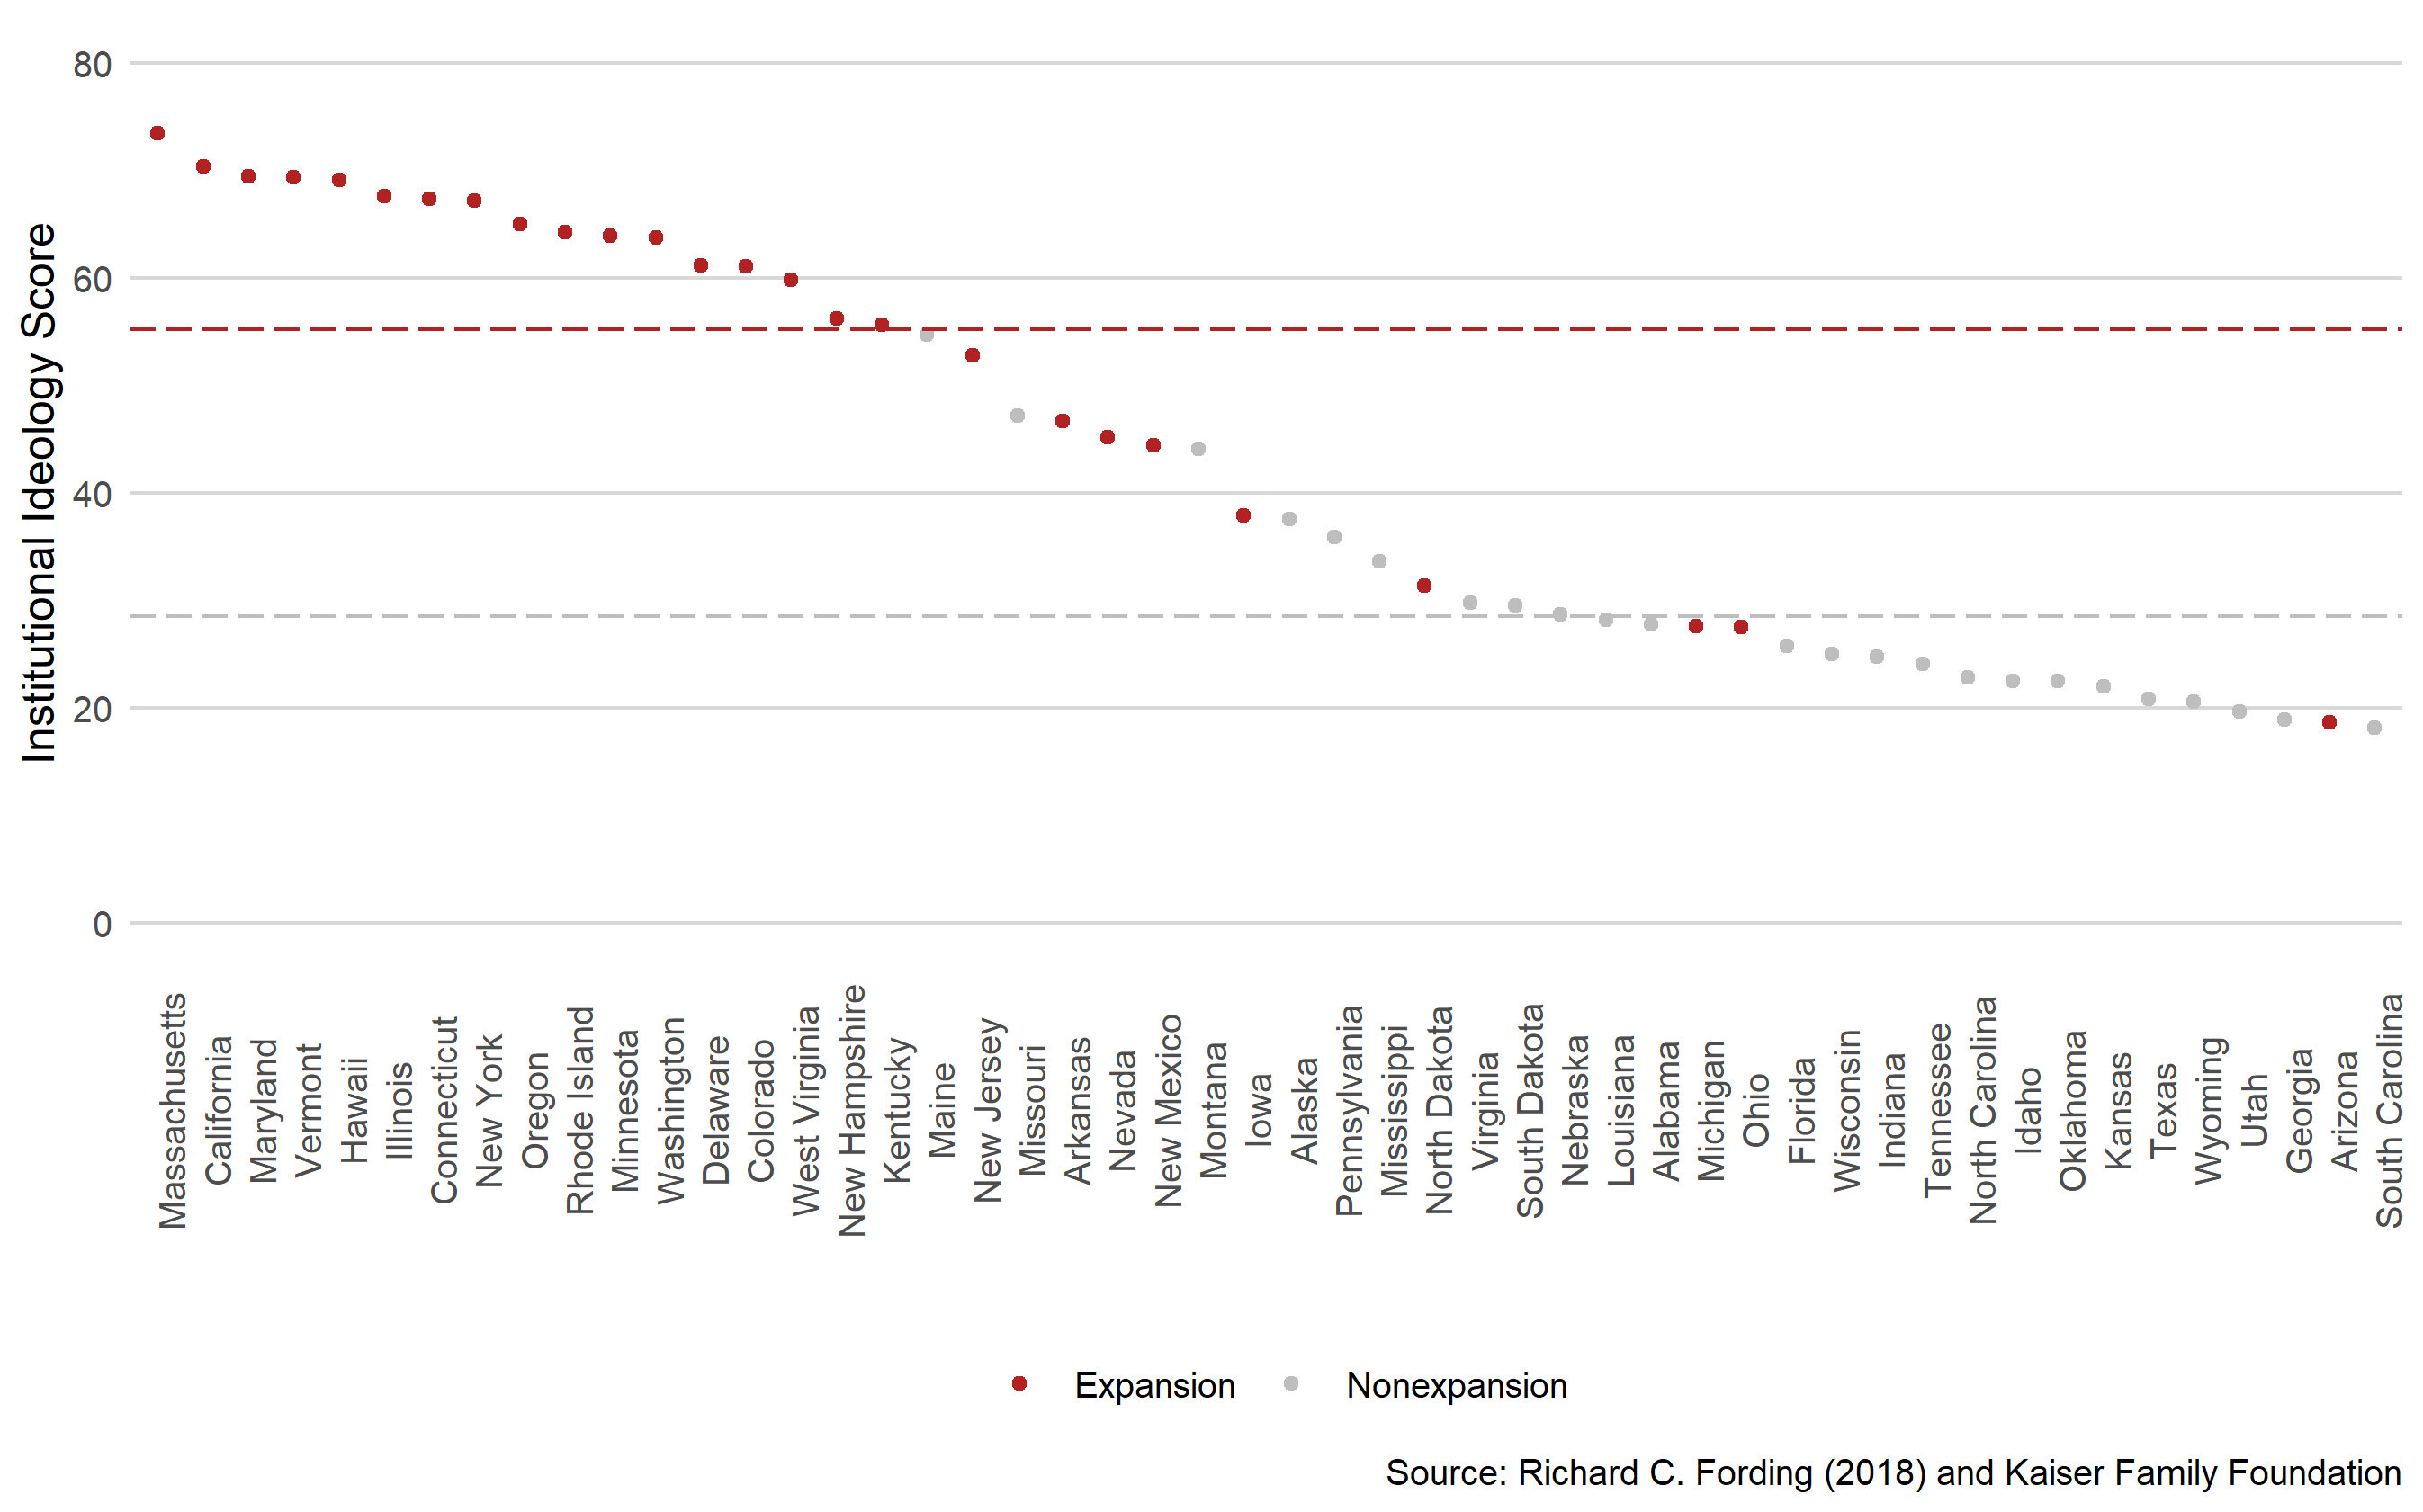
\includegraphics[bb = 0 scale=0.7]{political-expansion-plot.png}
%    \caption{Political ideology and Medicaid expansion}
%\end{figure}

Our results have broader implications for other potentially interesting effects. Insuring the previously uninsured is the primary mechanism that mediates most other effects of Medicaid expansion. We can therefore assume that if the ETU were closer to zero than the ETT, then further downstream effects that grow monotonically away from zero with the number of insured would also attenuate. For example, Wherry and Miller use their estimate of the ETT to project that had all states expanded Medicaid in 2014, XXX deaths would have been avoided. Assuming that mortality rates and uninsurance rates are negatively and monotonically related, we should expect this projection to be an overestimate. More generally directly estimating the ETU can help us to better model interesting downstream effects mediated through increasing the number of insured.

We have two goals in this paper: first, to estimate the ETU; second, to estimate the association between conservative governance and our estimate. We use survey data from 2011-2014 American Communities Survey (ACS) aggregated to the consistent public use microdata (CPUMA) level to estimate these effects. Existing panel-data methods typically use assumptions about stability over time to estimate counterfactuals absent treatment. By contrast we assume no unmeasured confounding and reweight our data to balance the covariates of the expansion regions to the non-expansion regions. We address four particular challenges in this paper: 

\begin{itemize}
    \item Treatment effect on the untreated: in the spirit of the synthetic controls literature, we reweight our treated units to match the untreated units in terms of their pre-treatment outcomes to estimate this effect, using an implementation of \cite{zubizarreta2015stable} Stable Balancing Weights to estimate these weights. However, the synthetic controls and differences-in-differences approaches rely on the stability of trends in the outcomes over time to impute the counterfactual outcomes absent treatment. By contrast, we are trying to estimate the treatment response, which may have rich dependence on the covariates. We therefore try to ensure that our model accounts for all possible sources of effect heterogeneity. This requires much stronger assumptions and does not admit data-driven covariate selection or placebo tests used in synthetic controls applications.
    \item Limited overlap: covariate overlap, particularly in terms of political partisan composition, is limited between expansion and non-expansion states. To improve our ability to balance our covariates, we estimate weights at the consistent public use microdata (CPUMA) level rather than the state-level. Even so, we are unable to get exactly balance, particularly on indicators of Republican governance. We therefore use outcome modeling to debias our estimates, at the cost of extrapolating beyond the support of the data and relying more heavily on outcome modeling assumptions. We check the robustness of these results by comparing the estimates to overlap weights (proposed by \cite{li2018balancing}) to estimate the overlap average treatment effect (OATE). 
    \item Variance estimation: valid variance estimation with aggregate panel-data is a much-studied but little agreed upon topic. However, all approaches we know of treat the covariate and treatment assignment values as known population quantities. Because our region-level values are estimates from underlying survey data, our approach to variance estimation takes into account this randomness and the randomness in the subsequent weighting process. However, our variance estimates do condition on the observed treatment assignment.
\end{itemize}

Section II provides an overview of our data, definitions and justifications for our study period, outcomes, treatment assignment indicator, and covariates. Section III is a broad overview of our methods, with three subsections on causal identification, statistical estimation, and inference. Section IV presents our results and some sensitivity analyses. Section V provides a brief discussion of the policy relevance of these. Supplemental materials may be found in the Appendix.

\section{Data}

Our data source is the annual household and person public use microdata files from the American Community Survey (ACS) from 2011 through 2014. The ACS is an annual survey of approximately three million individuals across the United States; the public use files include information on individuals in geographic areas greater than 65,000 people. The smallest geographic unit contained in these data are public-use microdata areas (PUMAs), arbitrary boundaries that nest within state but not within counties or other more commonly used geographic units. One limitation of these data is a 2012 change in the definition of PUMA boundaries; moreover, these new boundaries overlapped with the previous boundaries. As a result, the smallest possible geographic areas that nest both PUMA coding systems are known as consistent PUMAs (CPUMAs). The United States contain 1,075 total CPUMAs, with states ranging from having one CPUMA (South Dakota, Montana, and Idaho) to 123 CPUMAs (New York). The total number of sampled individuals per CPUMA in any year in our study ranged from 531 (representing an area of approximately 96,000 individuals) to 49,046 (representing over 4.5 million individuals). 

\subsection{Study period}

We start our analysis in 2011 following \cite{courtemanche2017early}, who note that several other aspects of the ACA were implemented in 2010 -- including the provision allowing for dependent coverage until age 26, and the elimination of co-payments for preventative care -- likely induced differential shocks across states. We also restrict our post-treatment period to 2014 only: several additional states expanded Medicaid in 2015, including Indiana, Michigan, and Pennsylvania. However, these states did not expand Medicaid contemporaneously with the 2014 ACA provisions. Therefore, this treatment is a different effect, unless we assume that the interaction effects between the ACA and Medicaid expansion are stable over time. 

\subsection{Covariates}

We use the underlying individual-level ACS survey data and accompanying survey weights to aggregate the data at the CPUMA level. We generate the following covariates for each CPUMA: total non-elderly adult population in 2011-2014; total labor force in 2011-2013; the total number of uninsured in 2011-2013; the total number of unemployed in 2011-2013; the total number of households (averaged). Among non-elderly adults, we calculate the total number of adults aged XXXX; total number of females; total number of whites; total number of foreign born; total number of citizens; EDUCATION; POVERTY; 

Finally, we include three variables reflecting a state's governance in 2013. Specifically, we include an indicator for having a Republican governor, an indicator for Republican control over the lower legislative chamber, and an indicator for Republican control over both chambers of the legislature and the governorship.\footnote{Nebraska is the only state with a unicameral legislature; moreover, the legislature is technically non-partisan. We nevertheless classified them as having a Republican control of the legislature.} 

\subsection{Outcome}

Our primary outcome of interest is the number of uninsured non-elderly adults. While the most natural outcome might be take-up rates among the Medicaid-eligible population, we choose this outcome for two reasons, one theoretic and one practical. First, Medicaid eligibility in the post-period is likely endogenous: Medicaid expansion may affect an individual's income and poverty levels, which define Medicaid eligibility. A second reason is to align our study to compare our results with the existing literature, and this is the outcome that \cite{courtemanche2017early} use. One drawback of using this outcome is that it is that the simultaneous adoption of other ACA provision in 2014 more clearly affects this total in a way that a more targeted group might not.

\subsection{Treatment assignment}

While some states expanded Medicaid and other states did not, assigning a binary treatment status is an oversimplification of the problem for three primary reasons. First, states differed substantially in pre-existing Medicaid coverage policies. With perfect data we might consider Medicaid expansion as a continuous treatment with values proportional to the number of newly eligible individuals. The challenge though is correctly identifying newly eligible individuals in the data (see \cite{frean2017premium}, who attempt to address this). Second, \cite{frean2017premium} note that six states adopted partial limited Medicaid expansions prior to 2014: specifically, California, Connecticut, DC, Minnesota, and New Jersey. \cite{kaestner2017effects} and \cite{courtemanche2017early} also consider Arizona, Colorado, Hawaii, Illinois, Iowa, Maryland, and Oregon to have had early expansions. Lastly, timing is an issue: among the states that expanded Medicaid in 2014, Michigan's expansion did not go into effect until April 2014, while New Hampshire's expansion did not occur until September 2014.

Our primary analysis excludes New York, Vermont, Massachusetts, Delaware, and the District of Columbia from our pool of expansion states, because these states had comparable Medicaid coverage policies prior to 2014 (\cite{kaestner2017effects}). We also exclude New Hampshire because it did not expand Medicaid until September 2014. While Michigan expanded Medicaid in April 2014, we leave this state in our treated pool. We consider the remaining expansion states as ``treated'' and the non-expansion states as ``control'' states. We later consider the sensitivity of our results to these classifications by removing the early expansion states noted by \cite{frean2017premium}. Our primary classification of expansion and non-expansion states is unique among similar studies: \cite{courtemanche2017early} classifies all expansion states as treated, and all non-expansion states as control. \cite{frean2017premium} exclude Massachusetts from expansion states. Lastly, \cite{kaestner2017effects} include Delaware, DC, Massachusetts, New York, and Vermont as control states, arguing that they were in some sense ``already treated.'' Our final dataset contains aggregated counts for all of the above variables for 925 CPUMAs in our non-expansion and our pool of expansion states. XXX CPUMAs were in non-expansion states and YYY CPUMAs are in expansion states.

\section{Methods}
\label{sec:methods}

We now outline our causal estimand, our identification and estimation strategies, and our inferential procedure.

\subsection{Estimand}

We seek to estimate the average effect of 2014 Medicaid expansion on the non-elderly adult uninsurance rate in states that did not expand Medicaid. As noted previously, the 2014 Medicaid expansion occurred simultaneously with the implementation of several other major ACA provisions, including (but not limited to) the creation of the ACA-marketplace exchanges, the individual mandate, health insurance subsidies, and community-rating and guaranteed issue of insurance plans \cite{courtemanche2017early}. Almost all states broadly implemented these reforms beginning January 2014. Conceptually we think of the other ACA components as a treatment ($V$) separate from Medicaid expansion ($A$).

Rather than rates, we begin by thinking about the total counts of uninsured non-elderly adults. Let $i$ index a CPUMA, $j$ index the state, $T = 2014$, and let $Y_{ijT}^{A_{ijT} = a, V_{ijT} = v}$ be the potential number of uninsured given Medicaid expansion and other ACA-reforms at time $T$. We consider the case where these potential outcome are deterministic: that is, given any state of the world $A = a, V = v$, a CPUMA has some deterministic potential number of uninsured non-elderly adults. Let $Y_L = \sum_{ij} Y_{ijT}$; that is, the total number of uninsured individuals across all CPUMAs and states at time $T$. We are interested in estimating the following contrast:

$$
\psi^L = \mathbb{E}\{Y_L^{A = 1, V = 1} - Y_L^{A = 0, V = 1} \mid A = 0, V = 1\}
$$

In other words, we want to estimate the difference in the total number of uninsured non-elderly adults among states that did not expand Medicaid, but did implement other aspects of the ACA. Because Medicaid expansion did not occur in any states that did not implement the ACA marketplace expansion in 2014, contrasts with the corresponding potential outcome are not identified. We then simplify notation by rewriting the estimand with $V$ as an effect modifier in the conditioning statement. Our estimand becomes:

$$
\psi^L = \mathbb{E}\{Y_L^{A = 1} - Y_L^{A = 0} | A = 1, V = 1\}
$$

This allows for interaction effects between Medicaid expansion and the rest of the ACA; however, we do not attempt to separately identify these effects. Notice that because non-expansion states were subject to an intervention the post-treatment period, in contrast to many other panel data settings, we do not observe $Y_L^{A = 0, V = 0}$ in the pre-treatment period. This has implications for standard identifying assumptions for the ETT. For example, parallel trends here requires that absent Medicaid expansion, the proportional change in the number of non-elderly uninsured adults would have been equal across expansion and non-expansion states. \cite{courtemanche2017early} build upon this assumption by using a DDD design; their identification assumes that the change in uninsurance rates would have been equal across areas with the same value of 2013 uninsurance rates conditional on other covariates. We assume that interactions between the ACA and Medicaid expansion may over time. Consequently, we do not seek to generalize these results outside of the context of the 2014 ACA implementation. .

Lastly, we need to convert $\psi^L$, which represents the change in the total counts, to $\psi$, which represents the more interpretable change in the uninsurance rate. We therefore treat the total observed 2014 population in each region as exogenous and divide our estimates of $\psi^L$ by this number. More precisely, let $P^L = \sum_{j: A_j = 0} p_{ij}$. Our final estimand is then:

$$
\psi = \psi^L/P^L
$$

The existing literature supports the assumption that these population counts are exogenous: CITE did not find evidence of migration across state lines due to Medicaid expansion. 

\subsection{Identification}

We make the following causal assumptions: consistency, no unmeasured confounding, no anticipatory treatment effects, and positivity of treatment assignment. Consistency states that the observed factual outcome under a given treatment assignment is equal to the potential outcome under that same treatment assignment ($Y_{ijt}^{A = a} = Y_{ijt} \mid A_{jt} = a$). In other words, we assume that regions that were not treated were affected by other states' treatment decisions. This assumption is standard throughout the literature, but often not realistic. This is true in our setting as well: \cite{frean2017premium} find evidence that Medicaid expansion drove previously eligible but uninsured individuals to enroll in non-expansion states. We do not test the sensitivity of our results to this violation, but note that it may impact .

We next assume that there were no anticipatory treatment effects. That is for $t \le T_0$

$$
Y_{ijt} = Y_{ijt}^0
$$

This assumption is necessary because we are conditioning on pre-treatment outcomes. If these outcomes were affected by the treatment before it were implemented, then they would not be exogenous. This assumption is also violated in our study: as noted above, several states had limited expansions prior to 2014. We are able to test the sensitivity of our results to the inclusion of these states.

Third, we assume no unmeasured confounding; that is the potential outcomes for each CPUMA are independent of the state-level treatment assignment conditional on CPUMA and state-level covariates $X$:

$$
Y_{ijt}^A \perp A_{jt} \mid X_{ijt}
$$

While unverifiable, we believe it is reasonable here given our rich covariate set. Additionally, conditioning on pre-treatment outcomes may help proxy for unobserved confounding (see, eg, \cite{abadie2010synthetic}).

Lastly we then assume positivity of treatment assignment; that is, that all CPUMAs had some probability of being treated $\pi(X_{ij}) > 0$. A lack of covariate overlap in the observed data can indicate potential violations of this assumption. We test for potential violations of this assumption by estimating the data-dependent overlap average treatment effect (OATE), proposed by \cite{li2018balancing}, in addition to the ETU.

\subsection{Estimation}

We estimate the ETU by using an implementation of Stable Balancing Weights (SBW) proposed by Zubizaretta (2015 (specifically, we use the ``optweight'' package in R). This procedure allows us to estimate the minimum variance weights that satisfy certain balance constraints. Letting $X_1$ and $X_0$ be the matrices of treatment and control group covariates (and dropping the subscript $t$ for notational simplicity), we solve the following objective function:

$$
\min_{w \in \mathcal{W}} \sum_{j: A_j = 1} w_{ij}^2
$$

$$
\mathcal{W} := \{w: n_c^{-1} \mid X_1^Tw - X_0^T1 \mid \le \delta, w_{ij} > 0, w^T1 = n_c\}
$$

We can then estimate $\psi^L$ as

$$
\hat{\psi}^L_w = (\sum_{j: A_j = 1}w_{ij}Y_{ij} - \sum_{ij: A_{ij} = 0}Y_{ij})
$$

Because we have balanced on the treatment group totals (and CPUMA means) of the covariates, we have implicitly assumed that our outcome model is linear and additive in these covariates. Specifically, we have that the outcome follows the following model:

$$
\mu_1(X_{ij}) = \mathbb{E}\{Y_{ij} \mid A_j = 1\} = X_{ij}^T\beta_1 
$$

The error of our estimator $\hat{\psi} - \psi$ is then equal to $\beta_1^T \delta = \beta_1^T(X_0^T1 - X_1^Tw)$ (see, eg, \cite{zubizarreta2015stable}). We then estimate this bias by regressing $Y_1$ on $X_1$ using OLS. This gives us a bias-corrected estimator:

$$
\hat{\psi}^L_{bc} = (Y_1^Tw - Y_0^T1 - \hat{\beta_1}^T(X_1^Tw - X_0^T1))
$$

Again the covariates and outcomes are all expressed in counts, though we really want to balance on the rates. We then divide both sides by the population among the control units $P^T$ to get:

$$
\hat{\psi} = \frac{\hat{\psi}^L}{P^L}
$$

This allows us to estimate the predicted change in percentage of non-elderly adult uninsured. 

By balancing on variables that include counts for the numerator and denominators for specific ratios, this procedure equivalently balances on the associated ratios. For example, we balance both on the total number of women and total number of non-elderly adults, this then balances the percentage of non-elderly adult women. Moreover, by balancing the numerators and denominators separately as counts for time-varying covariates, we ensure that when balancing the rates we are achieving the same changes within the numerators and denominators. Similarly, when estimating $\beta_1$, we express the covariates and outcomes in terms of CPUMA counts. 

We caveat that the way we have framed the balancing weights means that they are not conic rather than convex combinations of the expansion CPUMAs: this occurs in the requirement that the weights to sum to $n_c$ rather than $n_t$. On the other hand, we could have equivalently written the program to generate a proportional set of weights that sum to $n_t$, and these weights would be a convex combinations of the expansion CPUMAs. However, in this framing the total counts no longer balance. Because the number of CPUMAs in each group is an arbitrary standardization in any event, this framing is less interpretable, but it would give equivalent results.

Regardless, because we are ultimately interested in balancing rates, for the purposes of presenting our results we convert our covariates back into rates. While we used very tight balance constraints for the denominator counts, we did allow them to differ slightly. For both the covariates and the final outcome, we choose to present all of the results standardized to the same group's weighted denominator count rather than the targeted denominator count. This choice does not substantively effect the results. Full specifications of our targeted balancing constraints are available in the Appendix.

\subsection{Inference}

We take treatment assignment as fixed, and conduct inference with respect to the randomness in our estimate CPUMA-level covariates, outcomes, and our weighting procedure. In other words, if we actually observed the true CPUMA-level outcome and covariates, we would not present any confidence interval on our estimates in this framework.

To operationalize this inferential procedure, we use the 80 sets of replicate survey weights to generate 80 additional CPUMA-level datasets and we rerun the entire estimation procedure. These replicate survey weights account for the uncertainty in the survey weights we used to aggregate the data to the CPUMA level and take into account the complex survey design of the ACS. Where our original balance constraints become infeasible on the replicate datasets, we programatically reduce the balance constraints until we reach convergence. This program doesn't necessarily reflect exactly what we would have done had those been our starting datasets, but represents a reasonable approximation to the types of relaxations we may have conducted. We then estimate the standard errors as follows:

$$
\hat{\sigma} = \sqrt{\frac{4}{80}\sum_{b = 1}^{80}(\hat{\psi} - \hat{\psi}^B)^2}
$$

\section{Results}

Figure 1 visualizes balance results from our weights. We see that we were drastically able to reduce imbalances; however, several covariates remained largely imbalanced; in particular, the percentage of people living under Republican governance. 

\begin{figure}
    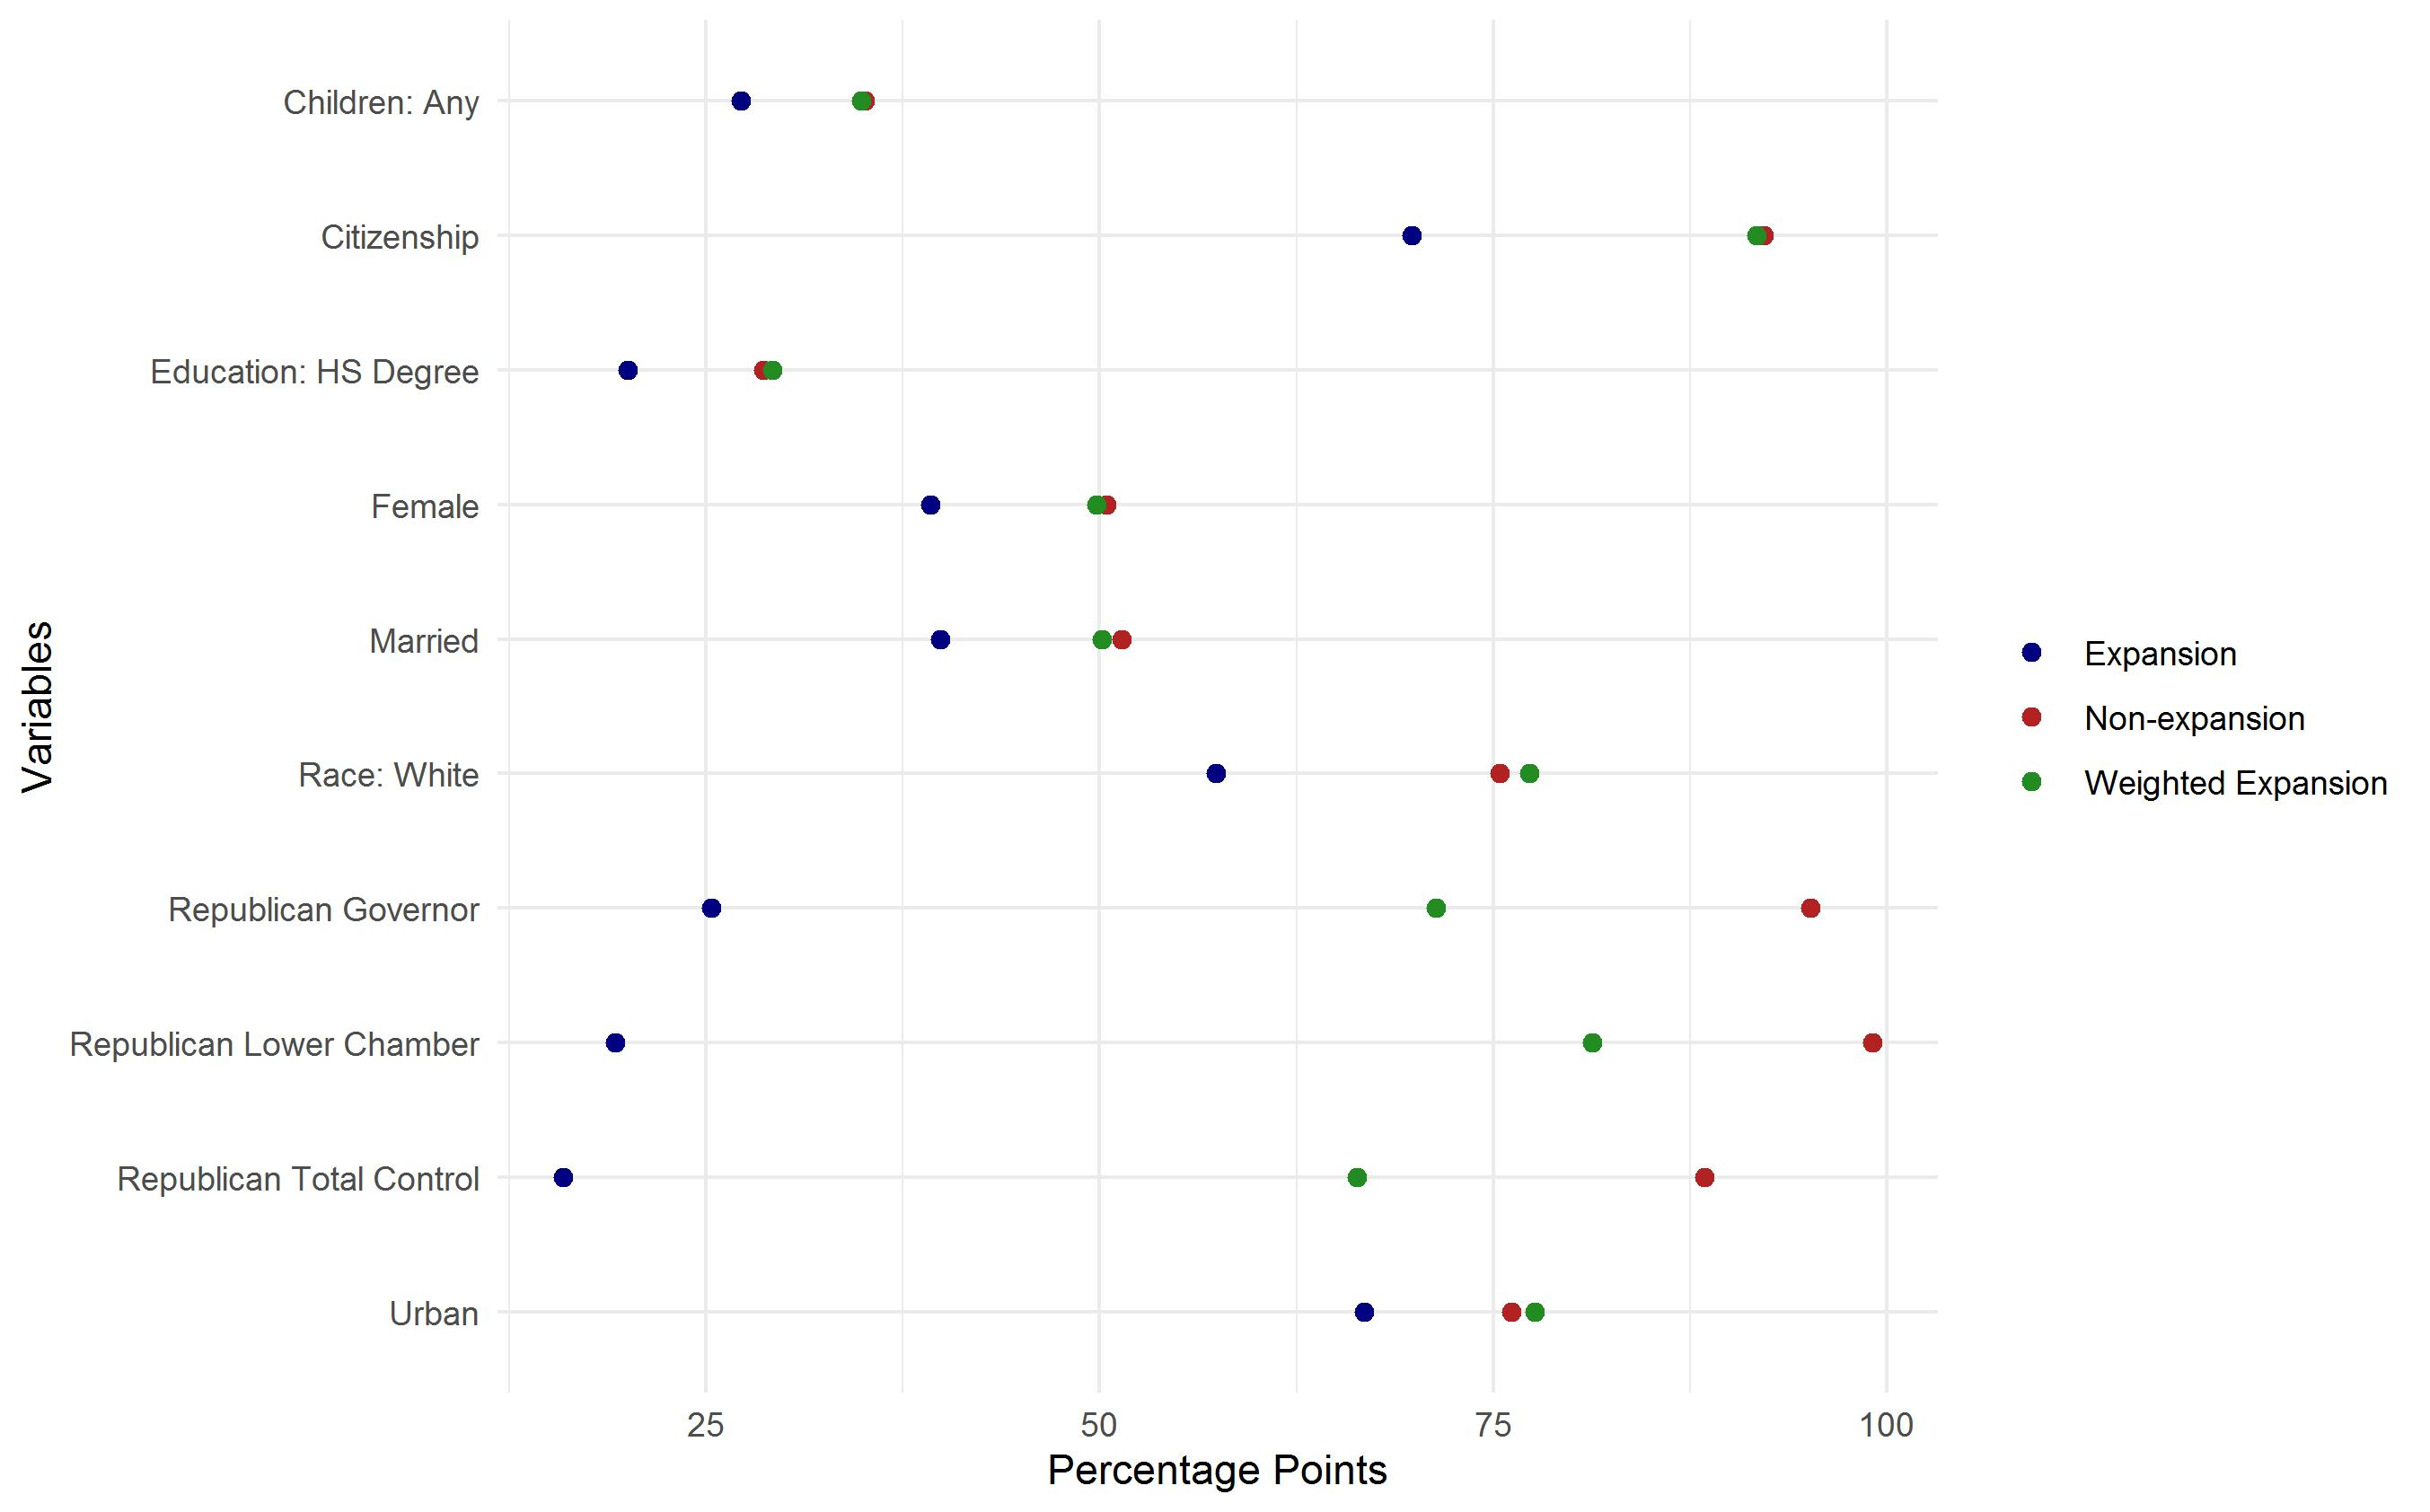
\includegraphics[bb=0]{images/balance-plot-largest10-unweighted.jpeg}
    \caption{CPUMA Weights by State}
\end{figure}

%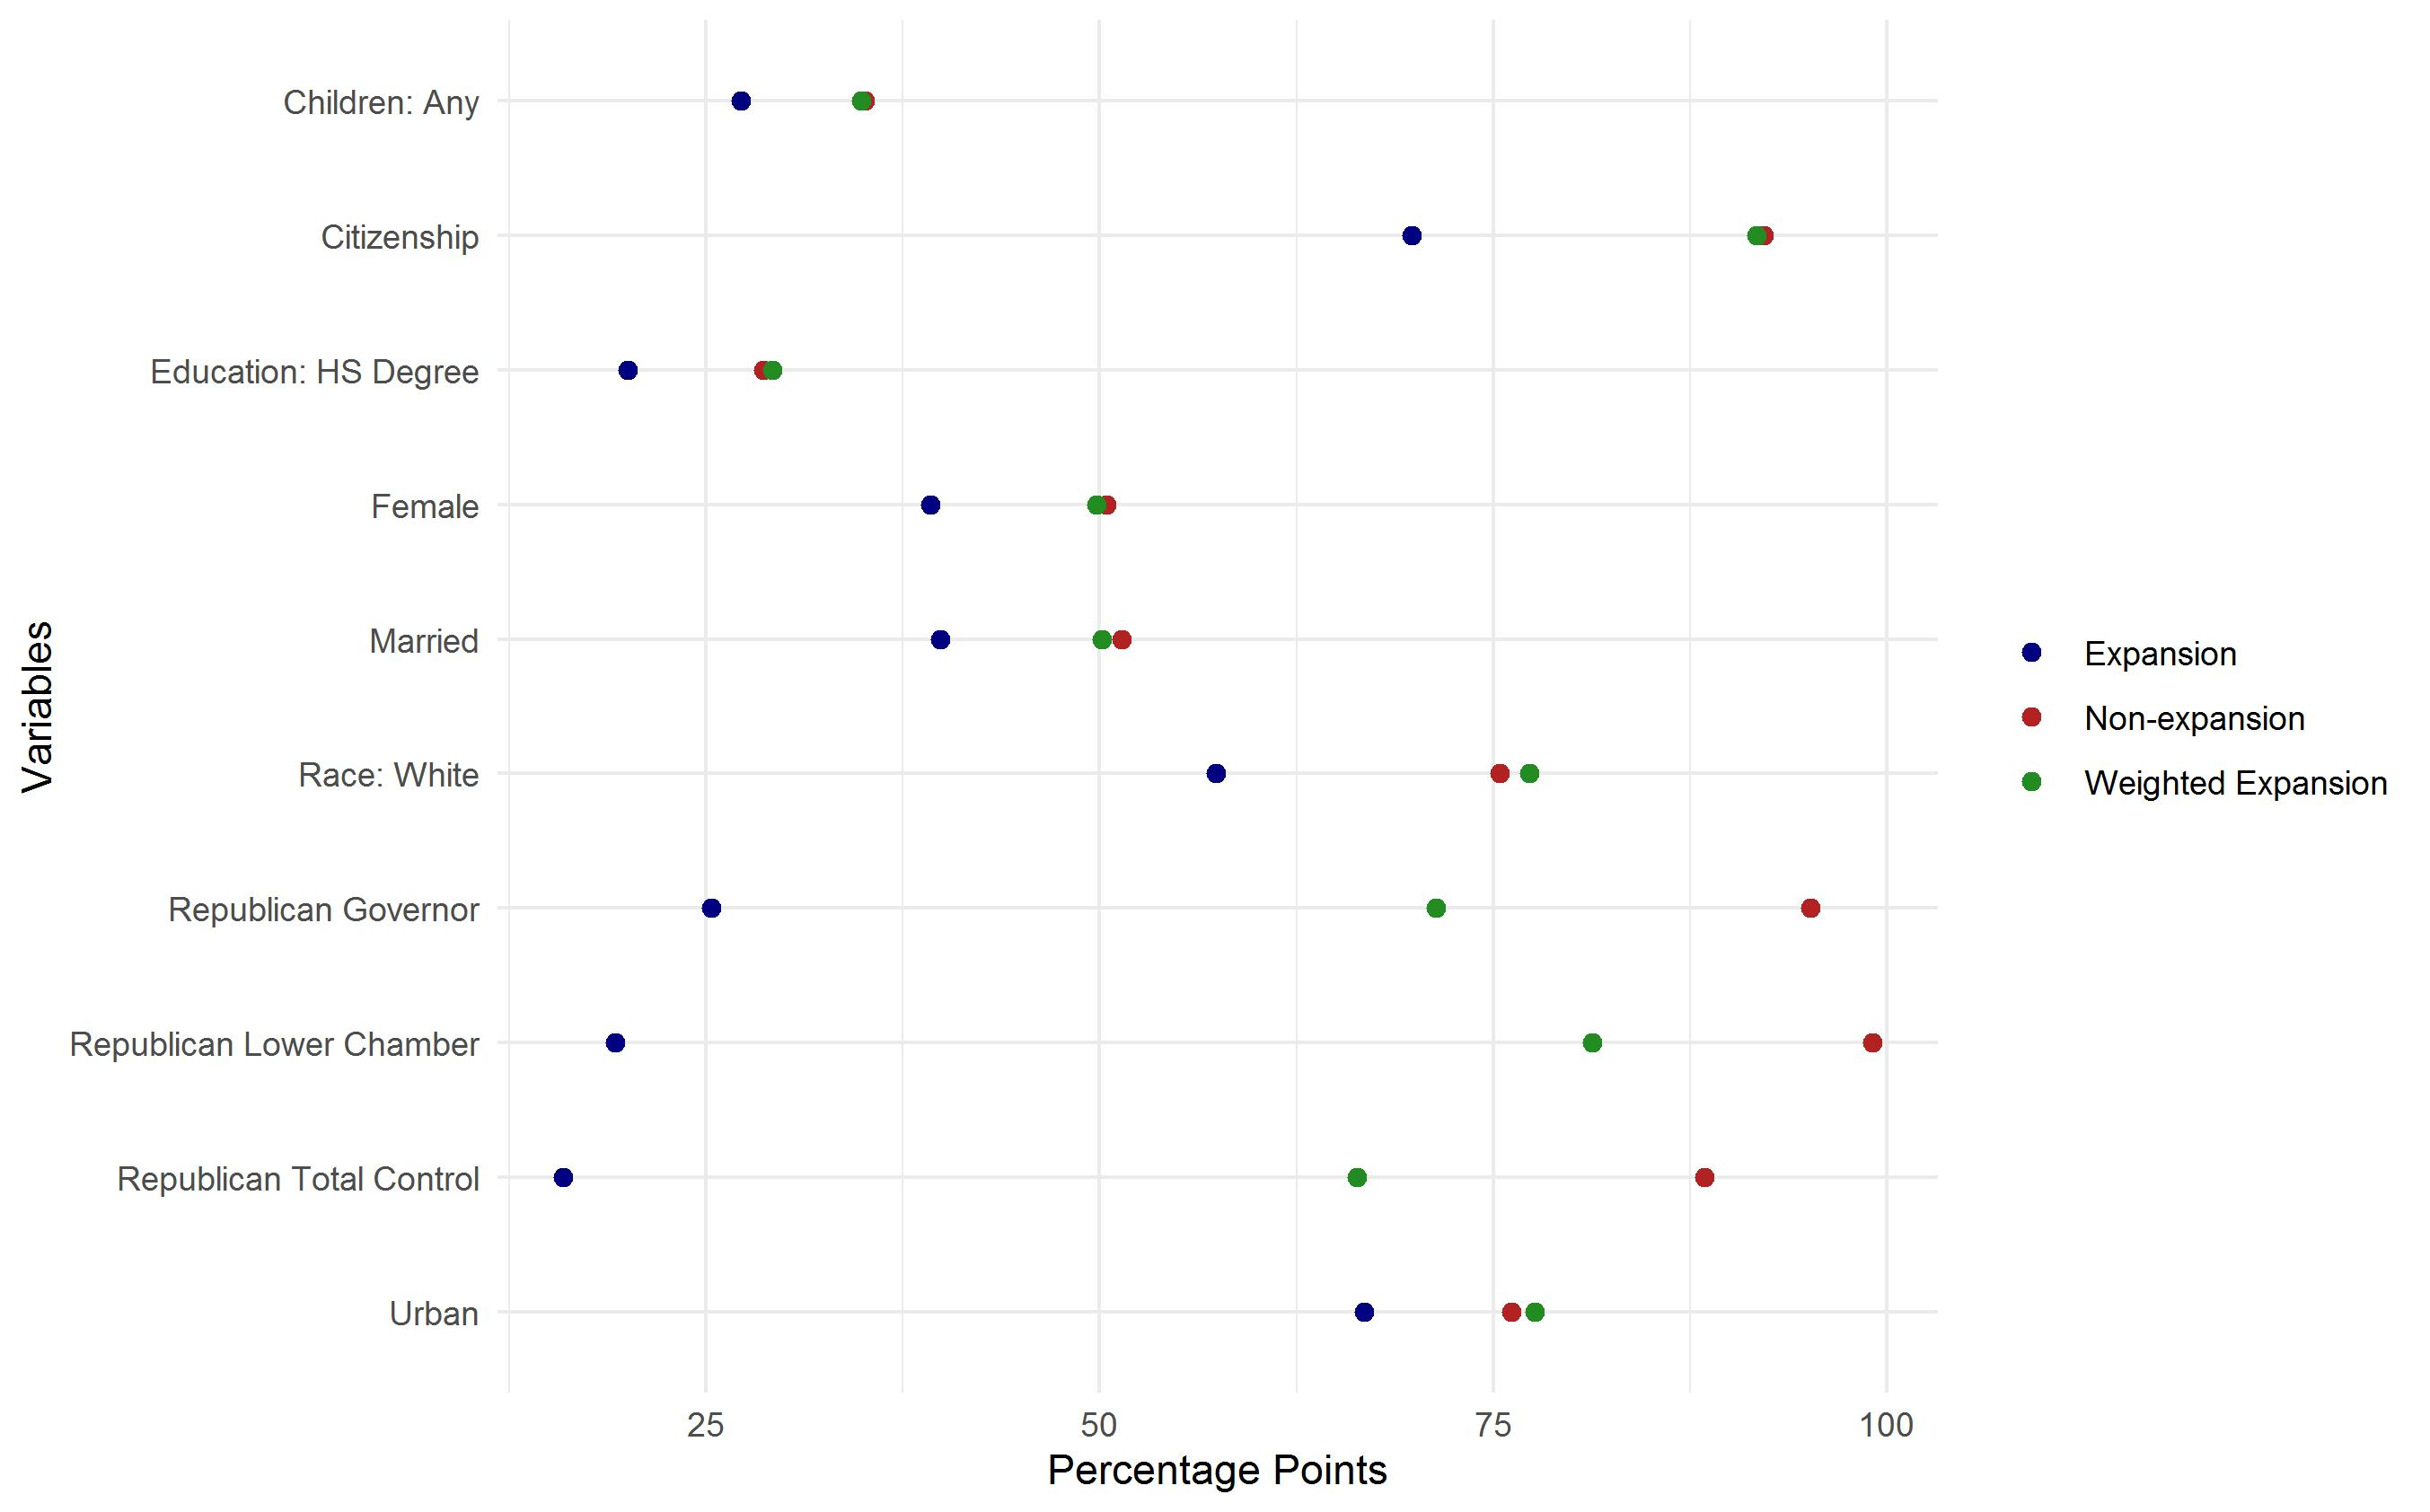
\includegraphics[bb=1]{images/balance-plot-largest10-unweighted.jpeg}

Figure 2 shows the CPUMA-level weights by state; within each states horizontal lines divide specific CPUMAs within the state. Since we balance on Republican governance, we see that several Democratic-controlled states receive close to no weight, including Colorado, Connecticut, Hawaii, Iowa, Kentucky, Minnesota, Oregon, Rhode Island, and West Virginia. On the other hand, we see that over half of the weights are attributed to CPUMAs between Arkansas and Ohio.

%\begin{figure}
%    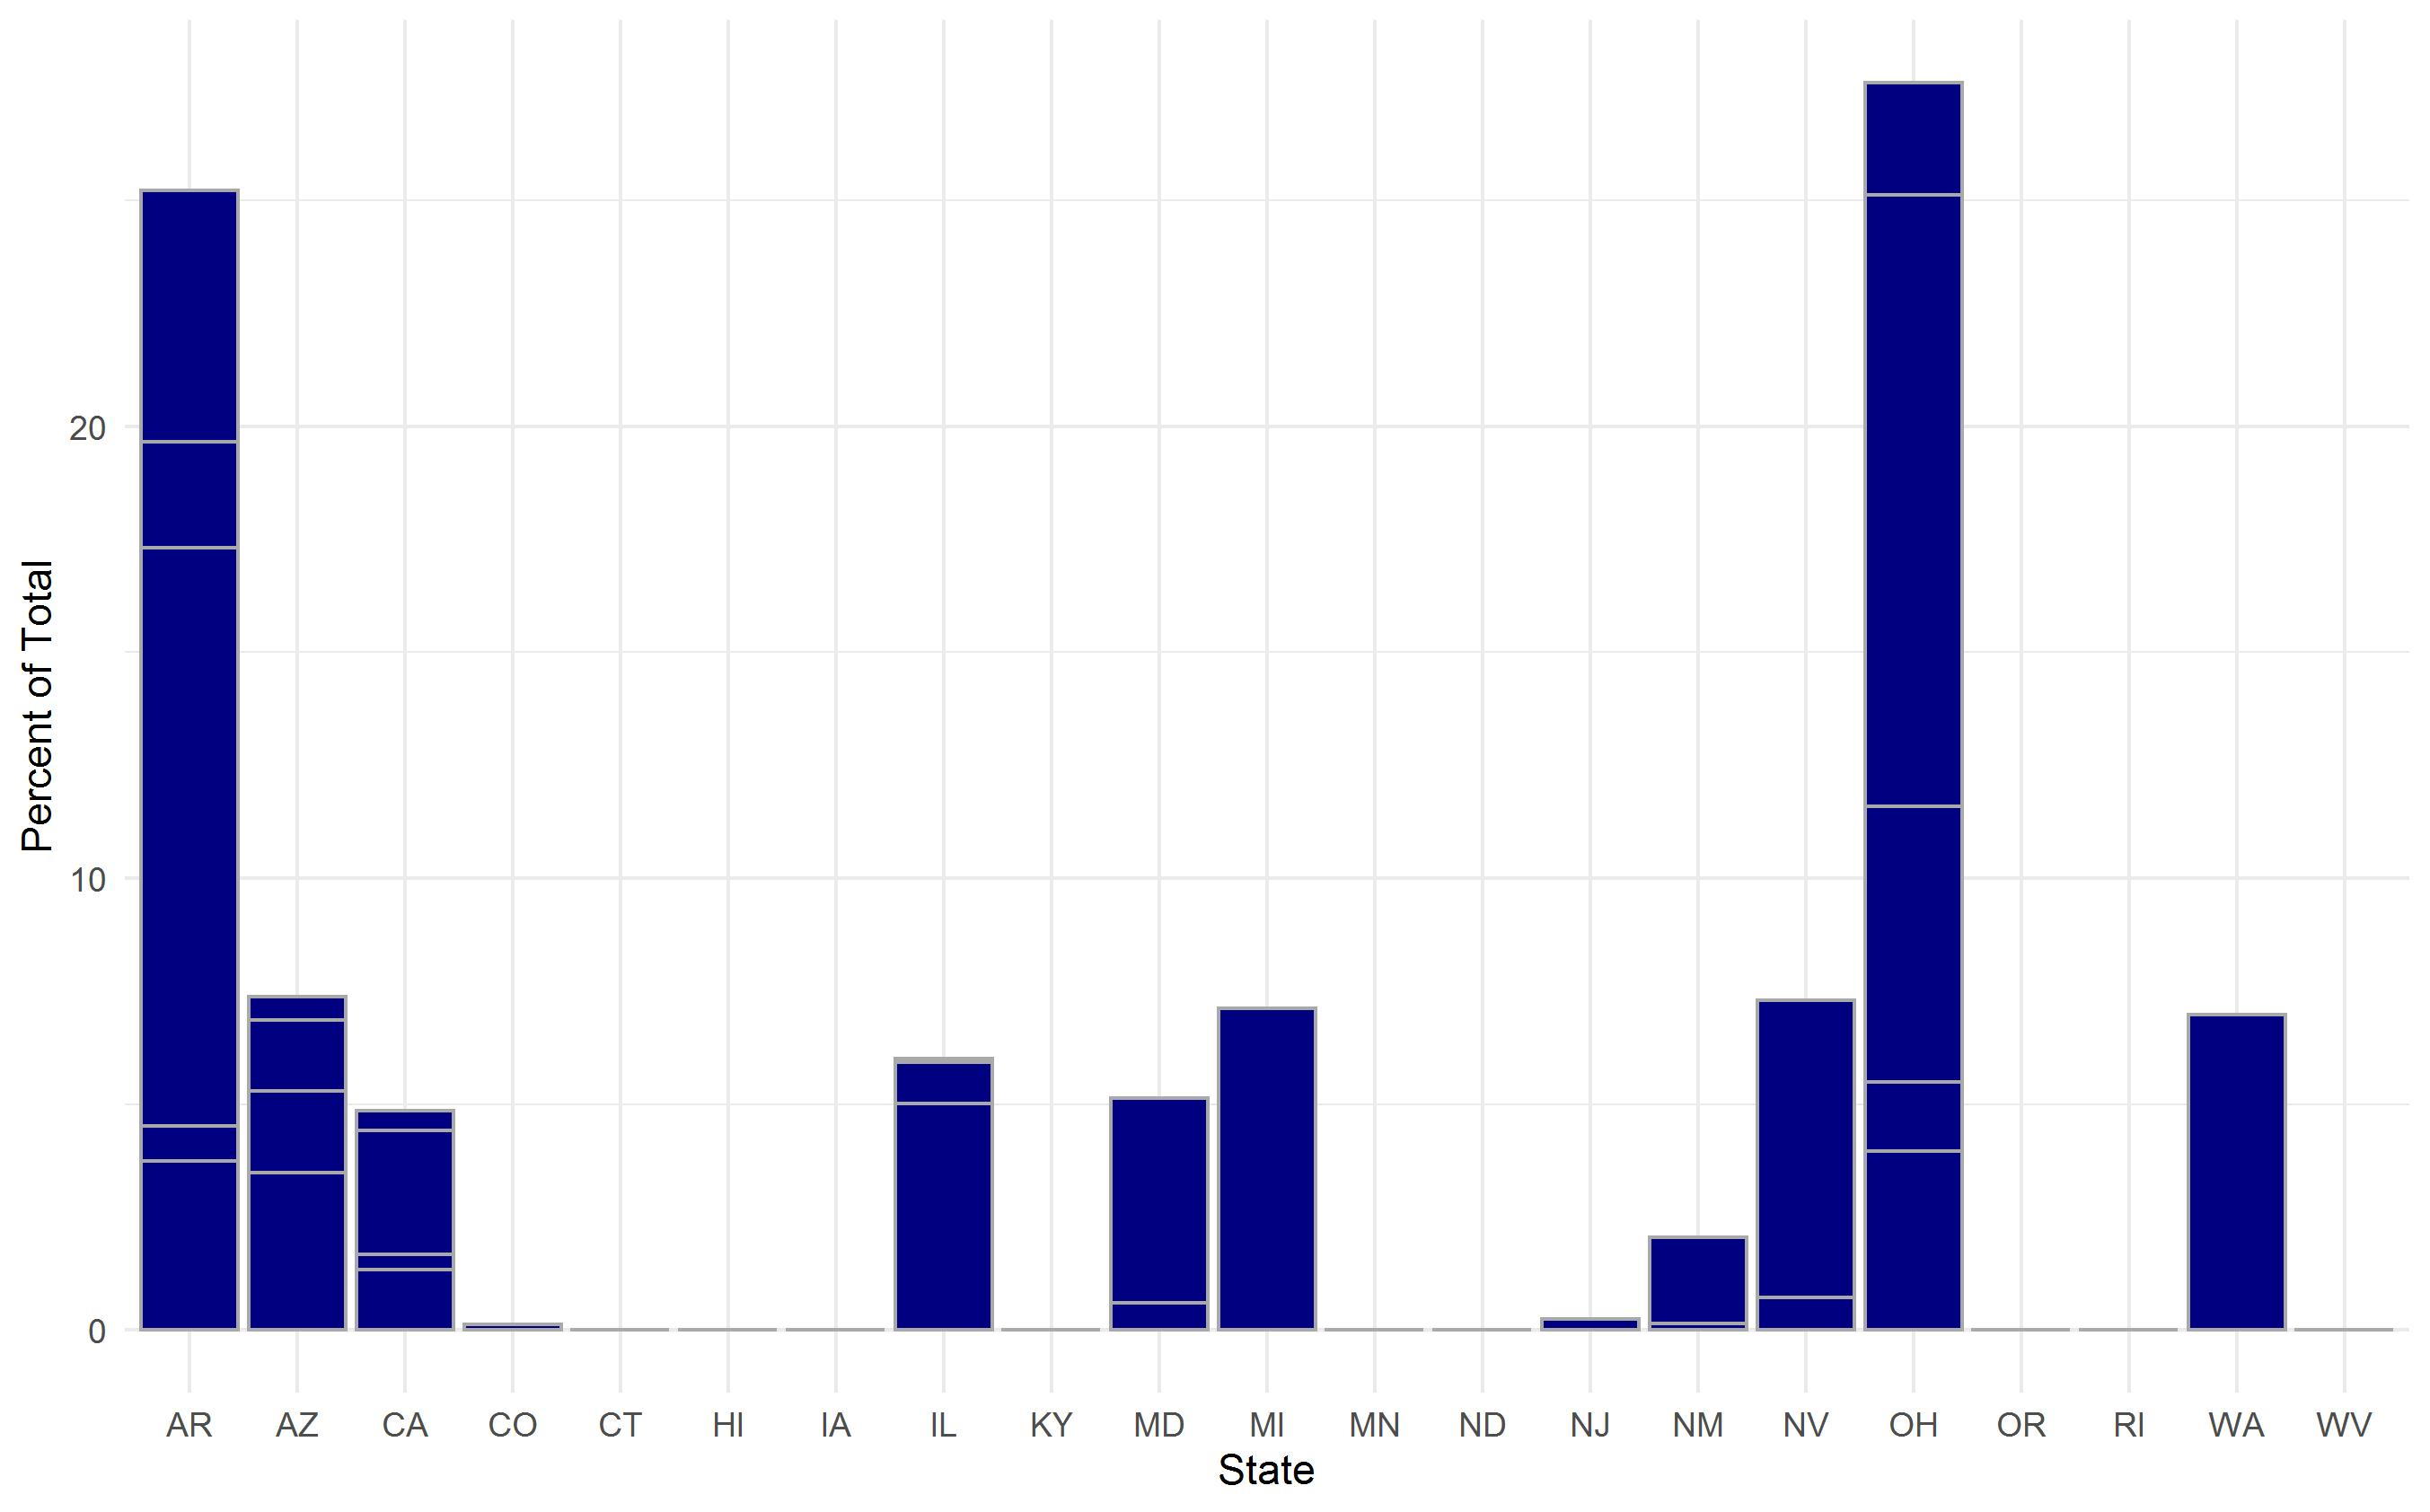
\includegraphics[scale=0.6]{cpuma-state-wgt-plot-new.png}
%    \caption{CPUMA Weights by State}
%\end{figure}

Using these weights we estimate a treatment effect of -2.21 (-1.32, -3.11). When we corrected for the remaining imbalances using a bias correction, we got a very similar estimate of  -2.18 (-1.31, -3.06). We emphasize that these confidence intervals account for the randomness in the estimation error for the CPUMA-level outcomes and covariates and in the weighting procedure. These confidence intervals therefore implicitly condition on the particular randomization we saw, and account for the sampling variability of our CPUMA-level covariate estimates and the weighting procedure alone. 

%\begin{figure}
%    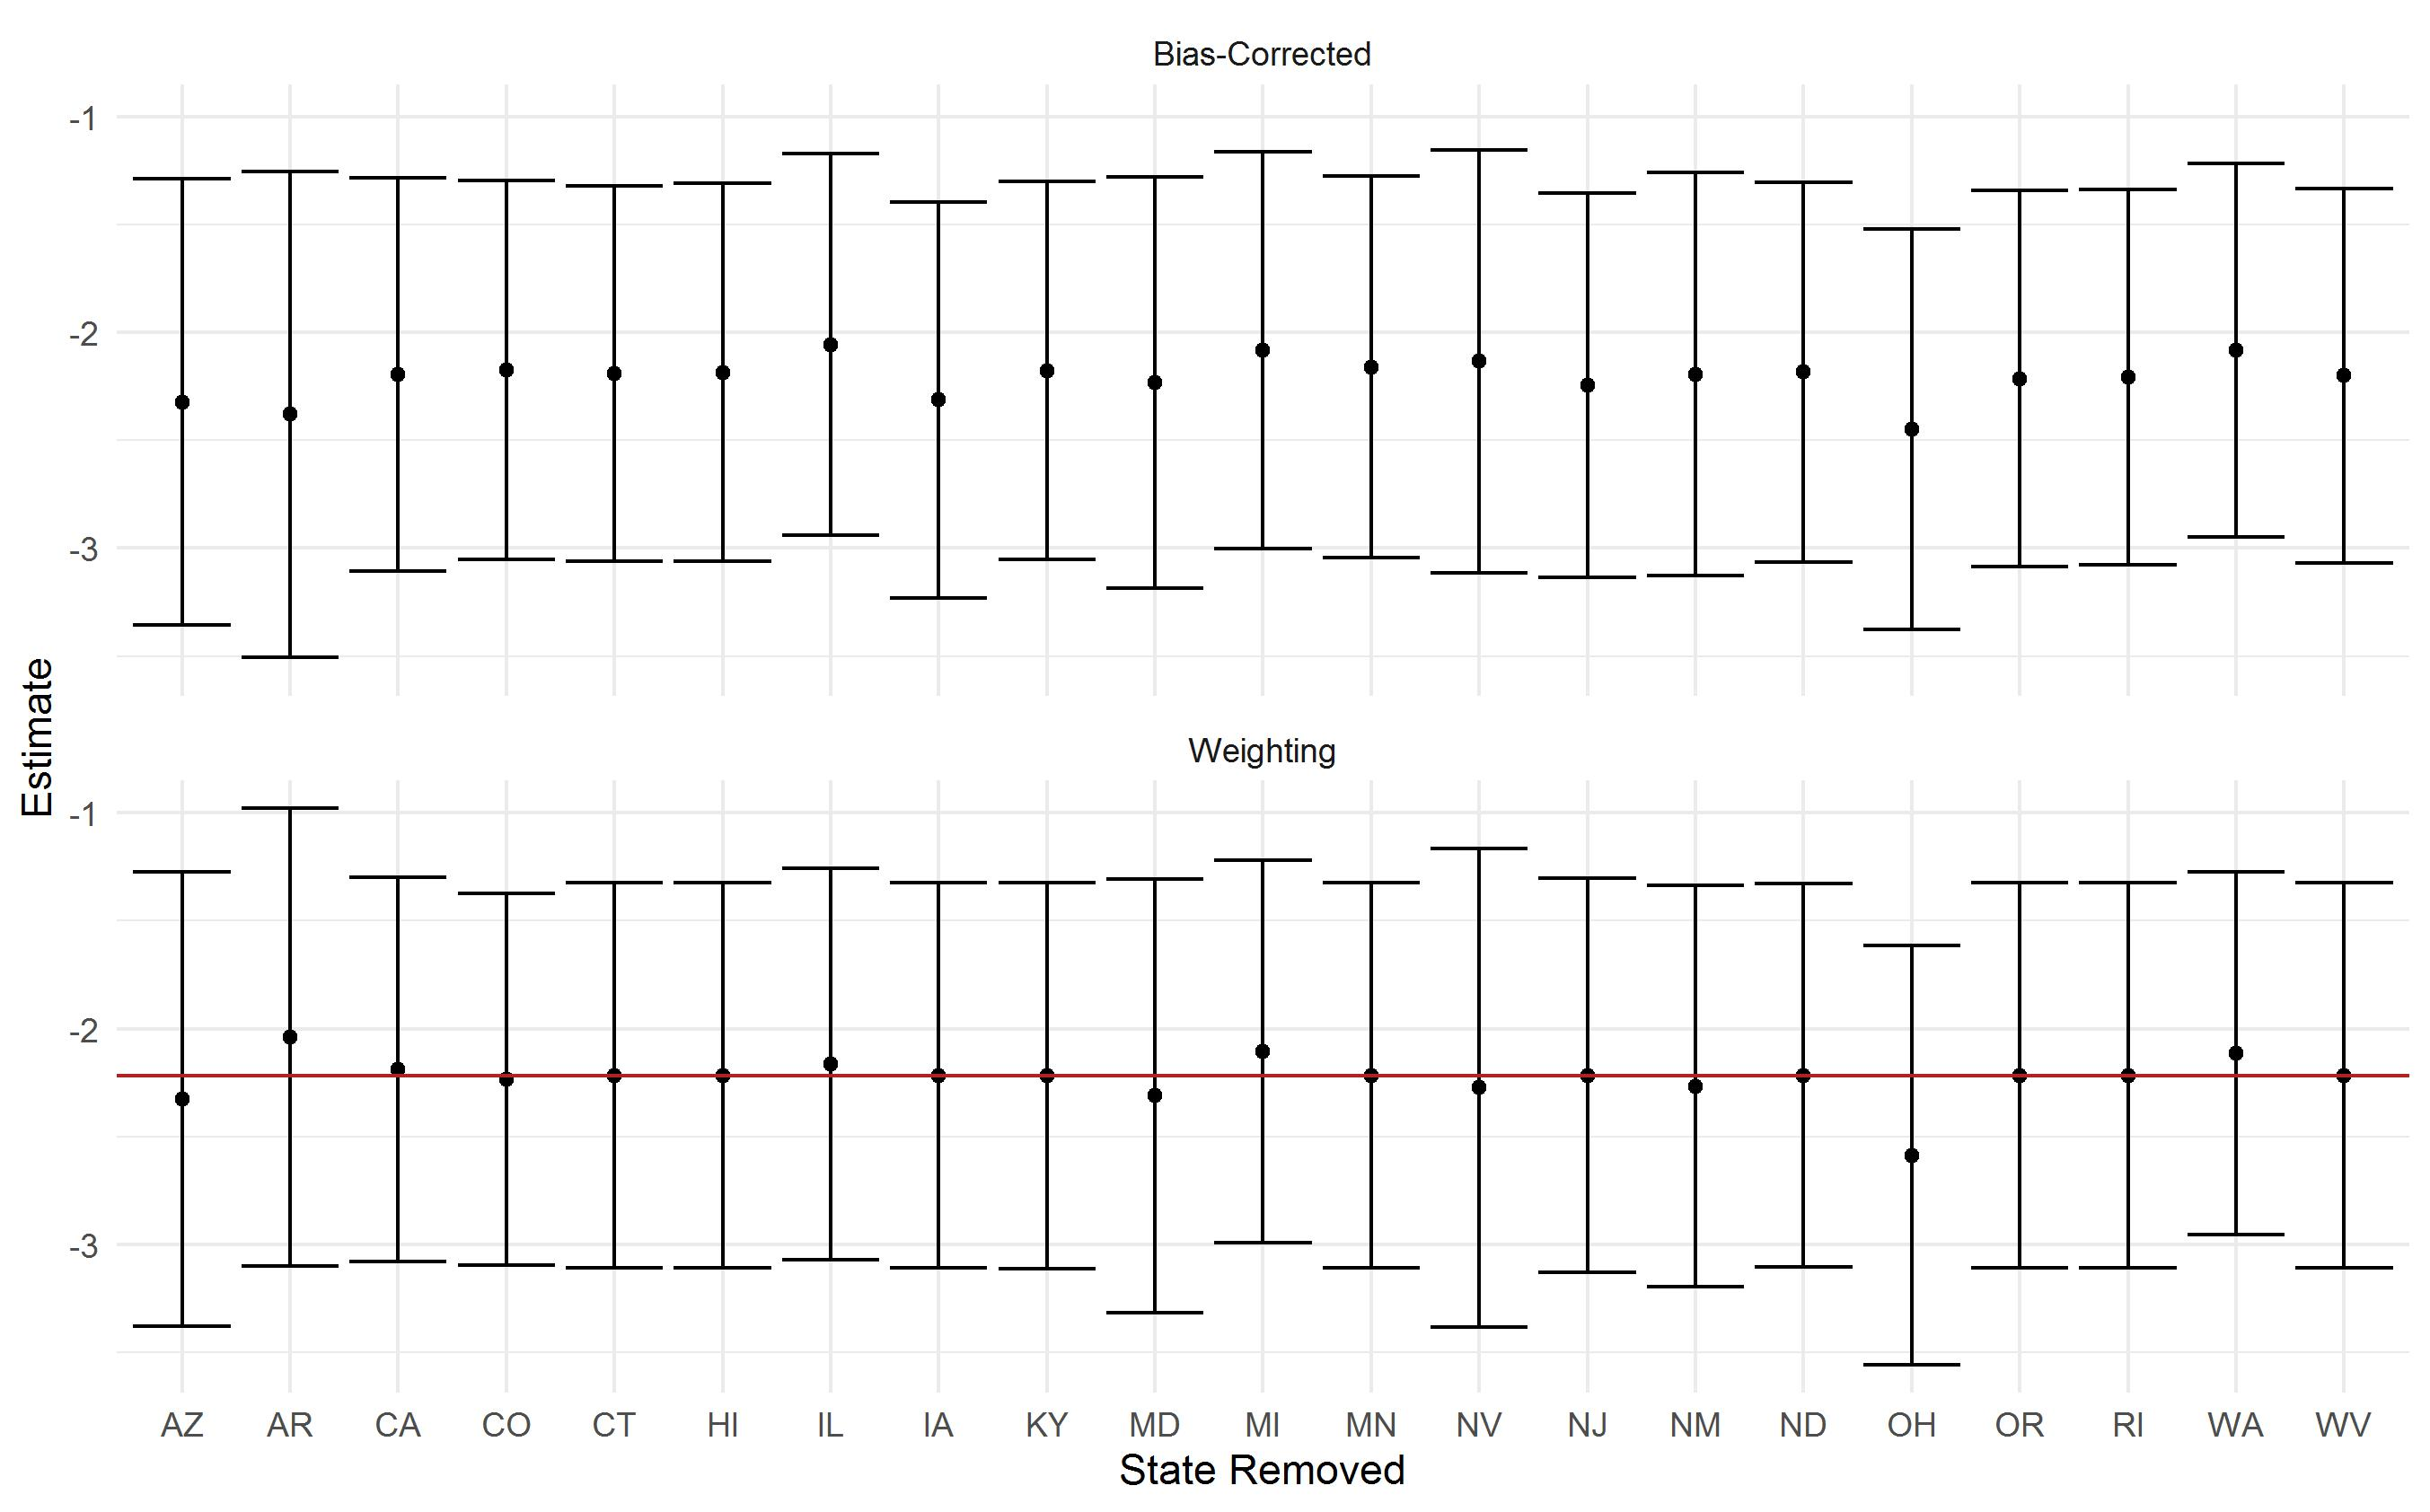
\includegraphics[scale=0.6]{loo-states-orig-dr.png}
%    \caption{Leave-one-out state analysis}
%\end{figure}

We examine how sensitive our estimates are to CPUMAs from particular states and remove one state at a time and rerun the procedure. Figure 4 presents the results for the the bias-corrected estimator (the weighting only results are similar and are available in the Appendix). Unsurprisingly, removing the states that received zero weights made no impact on our estimates. The results were somewhat sensitive to the exclusion of Arizona, Arkansas, and Ohio; in particular, the treatment effect moves further away from zero when we remove these states. Overall, we see that the results appear to be slightly less sensitive to the removeal of any particular state when when using the bias correction.

Our last analysis examines how important certain covariate groups are in determining these effects. We are especially interested how our treatment effects change when we remove the Republican governance indicators, since we hypothesize that this should be strongly associated with treatment effects closer to zero. We divide our covariates into six separate groups: pre-treatment uninsurance rates, pre-treatment unemployment rates, Republican governance indicators, racial demographics, education and poverty demographics, and other demographics (age, marital status, female, children, disability, student). We then rerun the analyses excluding each group. Figure YY displays the results. We see that removing the Republican governance indicators results moves the treatment effect estimates further away from zero, while the results are less sensitive to the other groups (results are similar when the weighting-only estimator and are available in the Appendix). 

%\begin{figure}
%    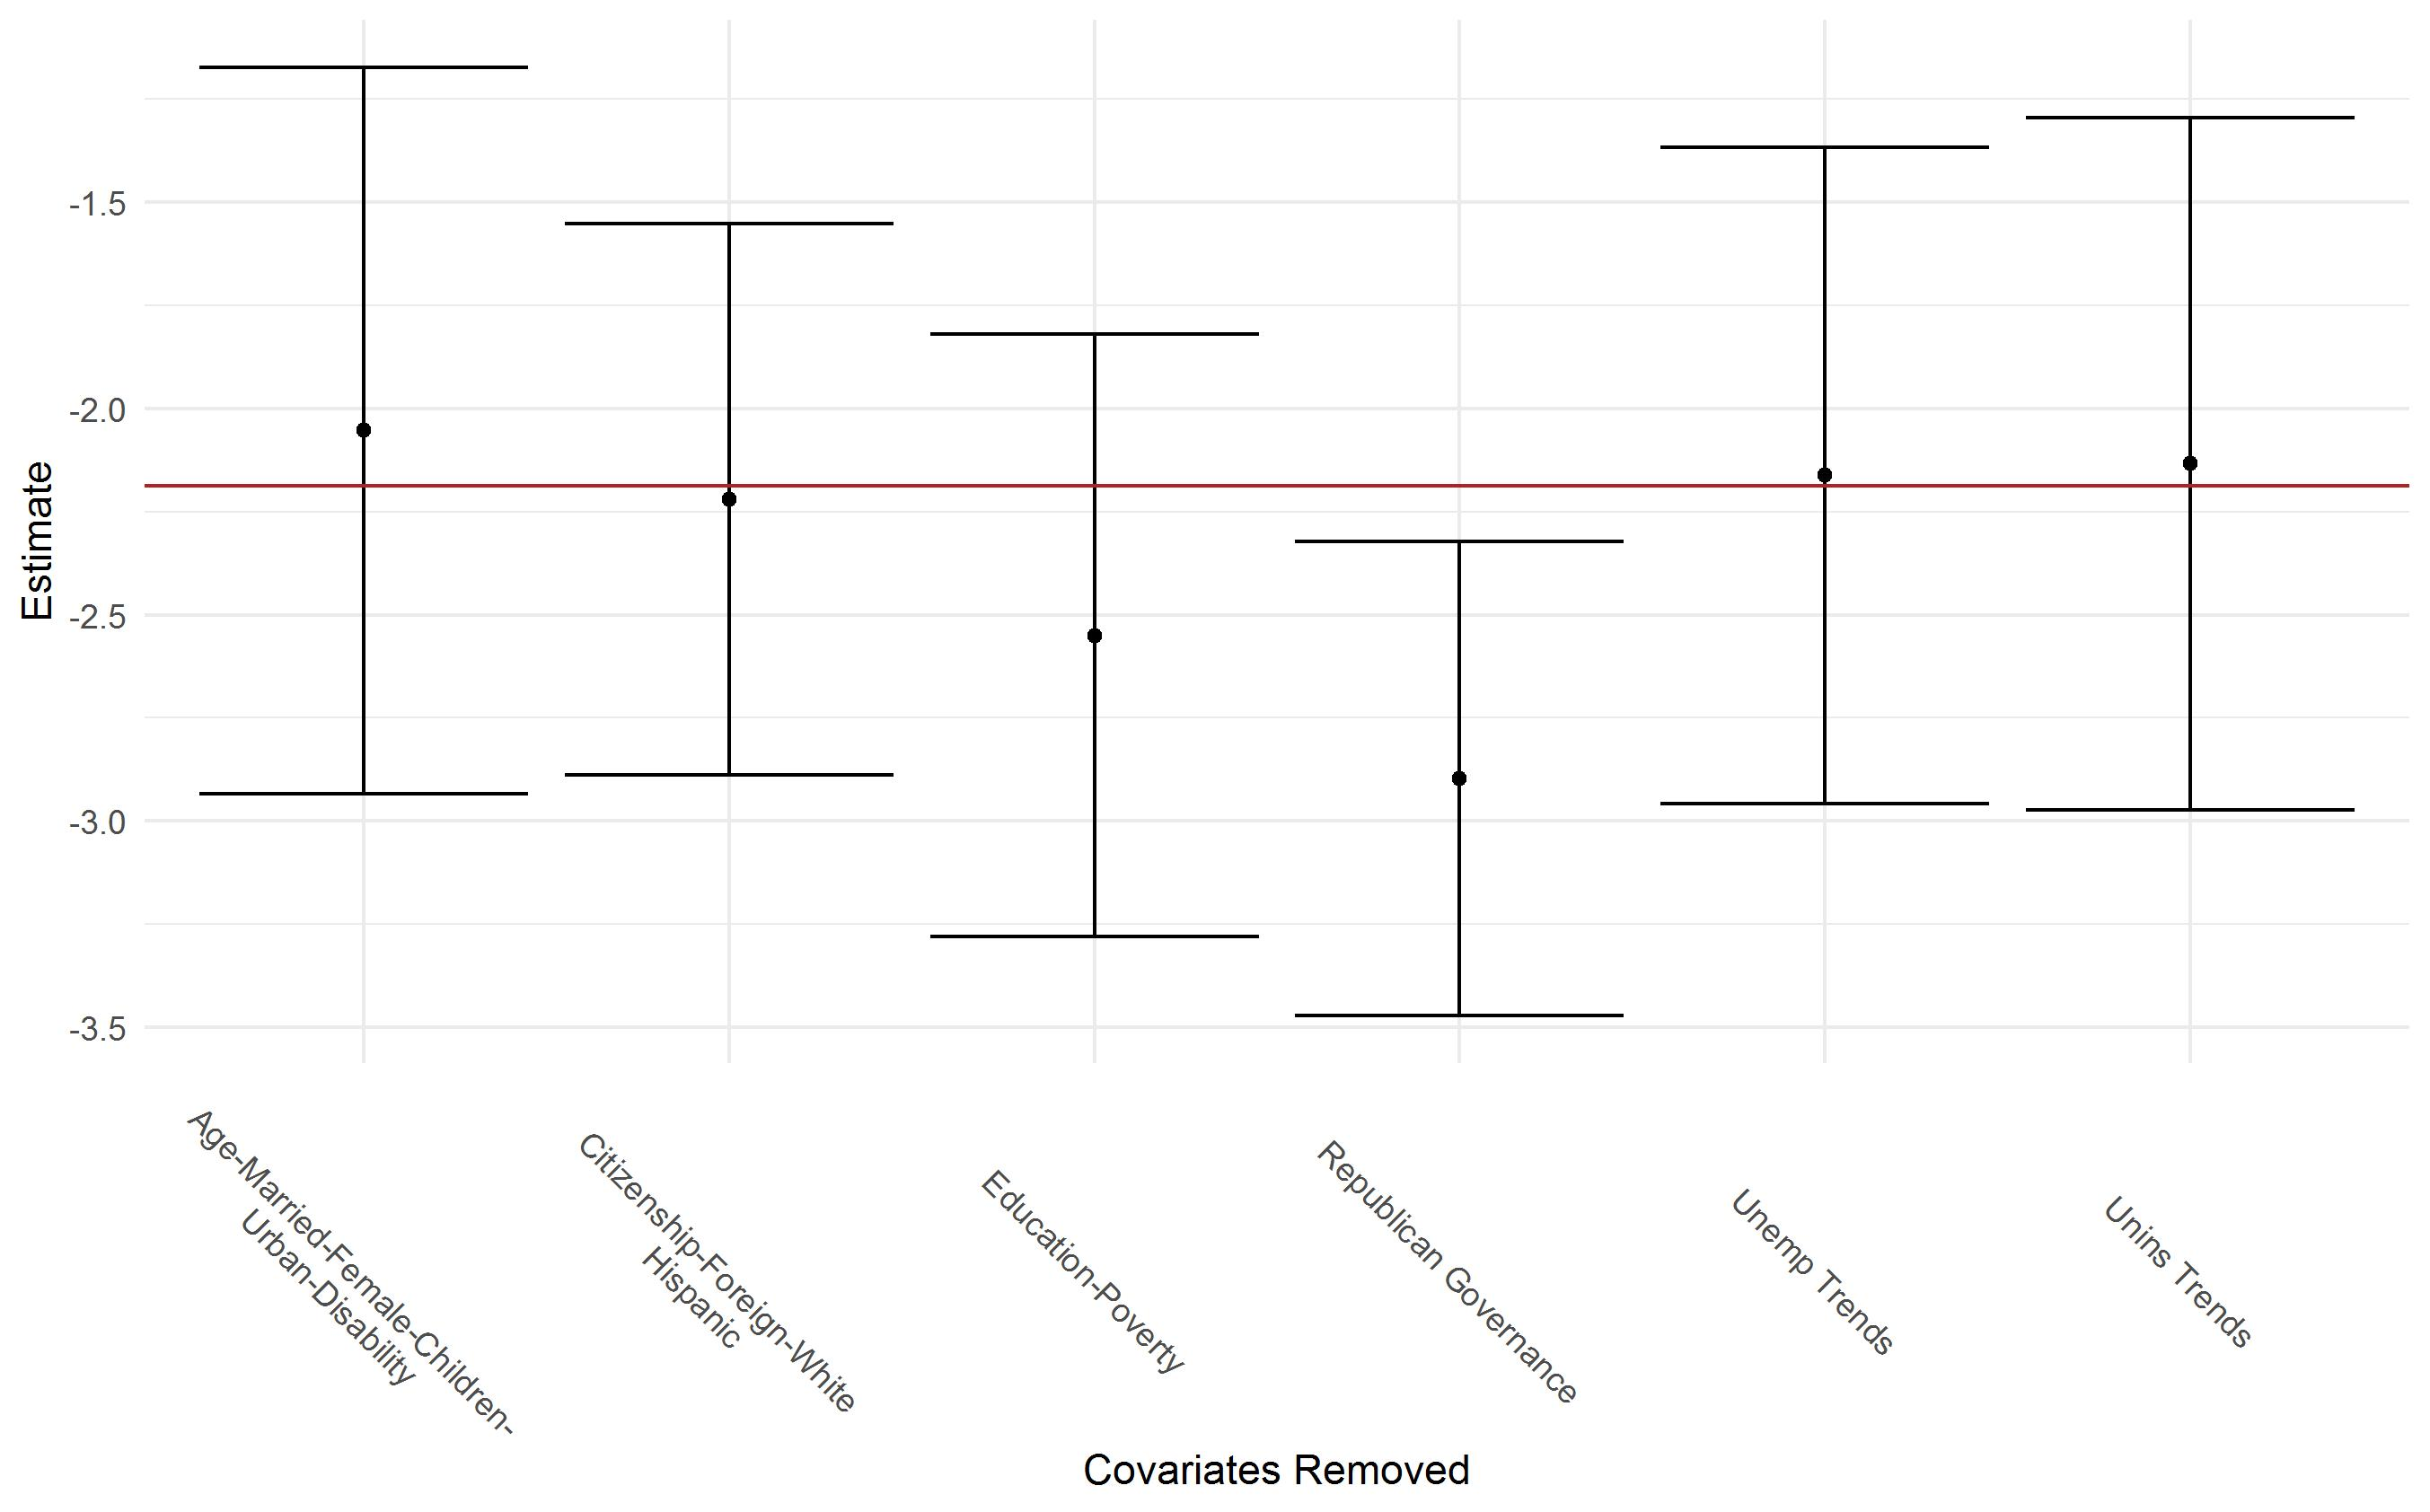
\includegraphics[scale=0.6]{loo-covariates-dr.png}
%    \caption{Leave-one-out covariates}
%\end{figure}

Overall these results suggest a strong relationship between the estimated treatment effect and Republican governance. However, CPUMAs from Ohio and Arkansas largely drive these estimates, and excluding these states may change this observed relationship. We therefore combined the leave-one-out covariate analysis with the leave-one-out state analysis to see how these estimated relationships changed. We find that this negative association between Republican governance and the estimated treatment effect holds even when leaving particular states out (results are available in the Appendix). This shows that no particular state drives these associations. 

\subsection{Sensitivity Analyses}

We next examine the sensitivity of our results to violations of two key causal assumptions: (1) no anticipatory treatment effects, and (2) positivity violations.

As we noted early, several states had partial limited expansions prior to 2014. Following \cite{frean2017premium}, we include California, Connecticut, Minnesota, New Jersey, and Washington in this group and rerun our analyses excluding CPUMAs from these states. We are unsure how we should expect this to affect our estimates: on the one hand, states that expanded early might have a smaller treatment effect after 2014 because they already enrolled newly eligible individuals. This would bias our previously estimated treatment effect upwards. On the other hand, if these states were also more motivated to enroll people in Medicaid, they might have larger post-exapnsion coverage gains, leading to a downwards bias. When removing these states, we estimate an effect of -1.97 (-0.96, -2.98). This is consistent with the latter story. However, when we run the bias-corrected version we estimate -2.27 (-1.48, -3.38), which is consistent with the former. Regardless, the confidence intervals largely overlap. Overall these results suggest that the bias from potential anticipatory treatment effects from these states was negligible. Our leave-one-out covariate analysis shows similar results to those in our primary analysis (results available in the appendix).

Our final analysis tests the sensitivity of our estimates to positivity violations. Because we were not able to get full overlap, our weighting estimators suffer some bias due to the imbalances, and our bias-corrected estimators rely on linearly extrapolating from our data. We therefore target the data dependent overlap treatment effect (OATE), using overlap weights proposed by \cite{li2018balancing}. Using logistic regression, we estimate the propensity scores and use these results to generate weights that exactly balance the means of the covariates between control and treatment group. This is essentially a data-drive method to implement commonly used weight ``trimming'' procedures. The cost is that we now have a data-dependent treatment effect: the OATE, which represents the treatment effect within regions where there is covariate overlap. We therefore are changing the target parameter.

Figure 8 shows the the expansion state, non-expansion state, and overlap weight covariate means, ordered by the largest difference between expansion and non-expansion states. We see that the overlap region is in general closer to the non-expansion states. This is a more conservative, less diverse region. Interestingly, we also see that the pre-treatment uninsurance and unemployment rates are also lower than either the overall expansion or non-expansion states. We find that the average L2 distance between the expansion states and overlap region is 8.29 percentage points while it is only 2.91 between the non-expansion and overlap region. This suggests that we should think of the OATE as substantially closer in spirit to the ETU than the ETT.

Figure 7 shows the total percentage contribution of CPUMAs within each state to the overall OATE weights by treatment group. Notice that many of the expansion states are heavily downweighted, whereas the distribution across the non-expansion states is more uniform. In particular, we see that Ohio and Michigan constitute over 50 percent of this regions weights, while the Pennsylvania, Wisconsin, Missouri, and Florida represent over 50 percent of the non-expansion state weights.

%\begin{figure}
%    \includegraphics[scale=0.6]{overlap-weights-state-weights-Preferred.png}
%    \caption{OATE Percentage Weights by State}
%\end{figure}

We estimate that the OATE is -2.02 (-1.63, -2.41). This result is virtually unchanged when we remove the potential early expansion states, giving an estimated effect of -2.01 (-1.61, -2.40). Figure 8 shows that results are quite insensitive to removing any particular non-expansion state, though they appear most sensitive to Ohio, Iowa, and Arkansas. Our leave-one-out covariate group again shows the negative association between Republican governance and the magnitude of the treatment effect. The leave-one-out covariate group by state analysis is available in the Appendix and is consistent with these results, again showing that Republican governance is negatively associated with the estimated treatment effect.

%\begin{figure}
%    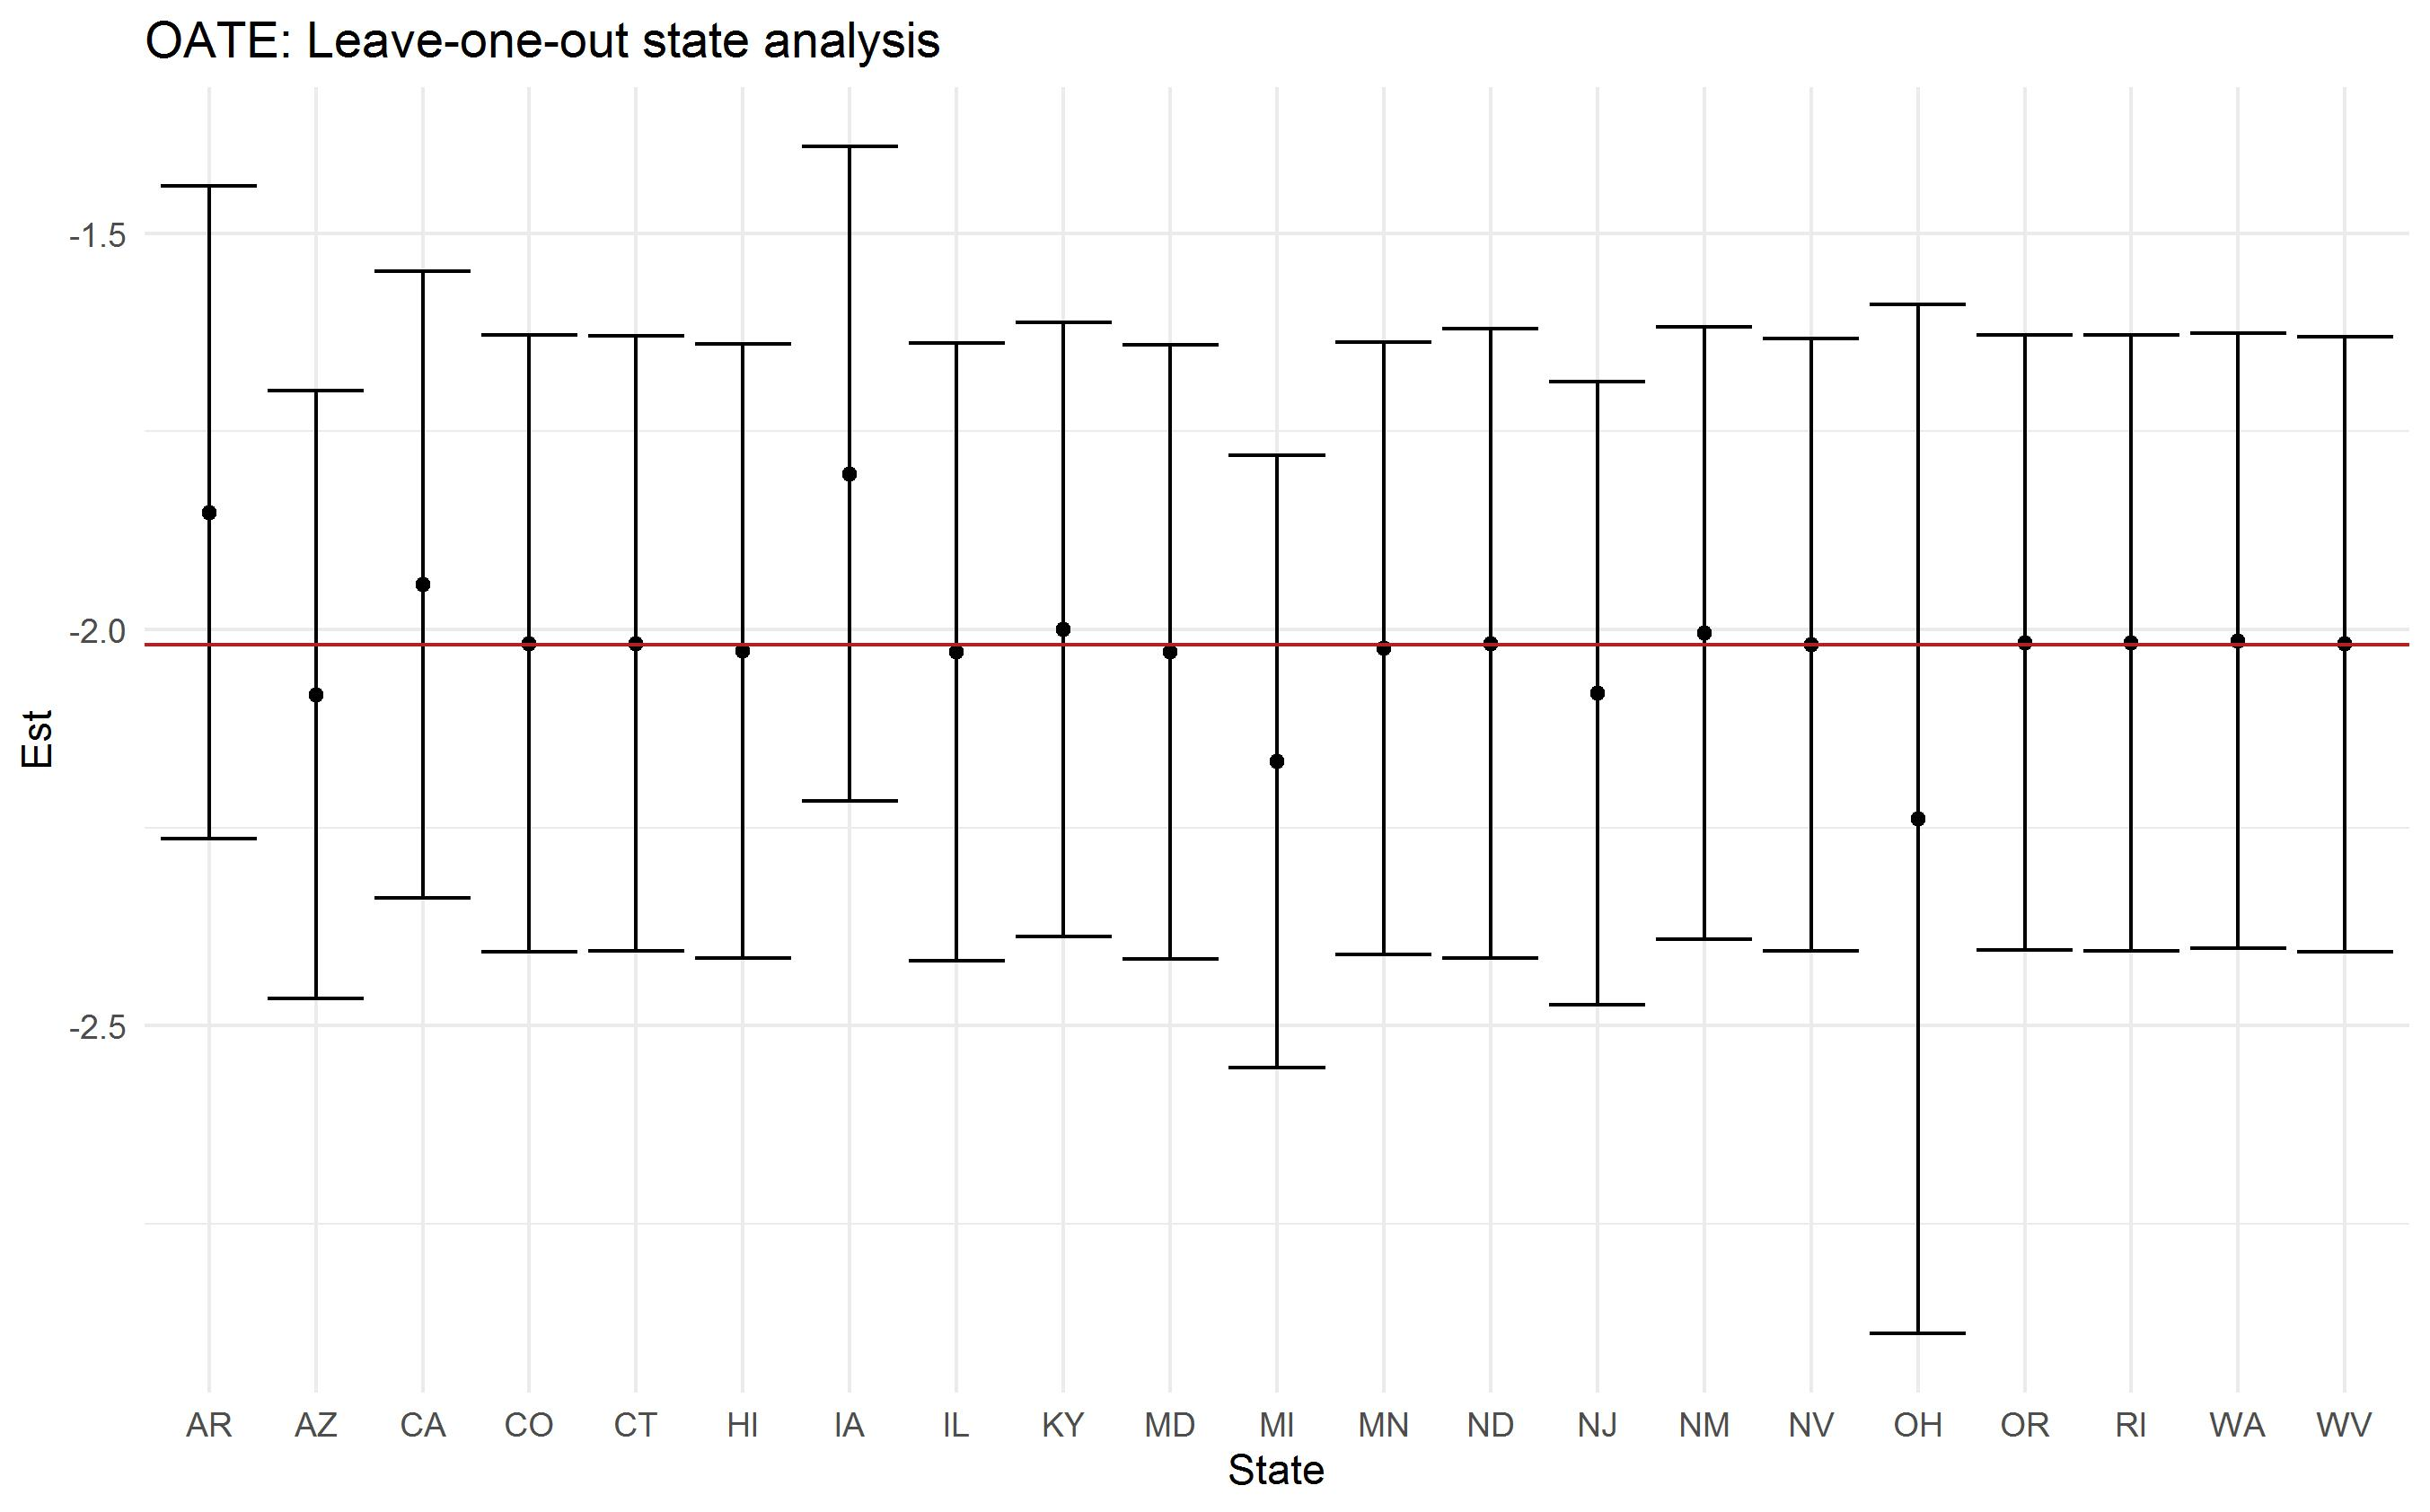
\includegraphics[scale=0.6]{oate-loo-state.png}
%    \caption{OATE Leave-one-out state analysis}
%\end{figure}

\section{Discussion}

This is the first study to directly estimate the foregone coverage gains of Medicaid expansion among states that did not expand Medicaid. Our best estimate is that these states would have seen their uninsurance rates decrease by -2.18 percentage points (-1.31, -3.06) in 2014 had they expanded Medicaid in 2014. We also find a consistent negative association between our estimates and Republican governance. Given the Democratic political composition of states that expanded Medicaid, this suggests that we should expect the ETT to be further away from zero than the ETU. This finding is also consistent with the existing literature, which places estimates of the ETT between three and six percentage points (\cite{kaestner2017effects}, \cite{courtemanche2017early}, \cite{frean2017premium}), and which also finds lower Medicaid take-up rates prior to expansion in 2014 among conservative states, even after controlling for other variables (\cite{sommers2012understanding}). These results are not sensitive to any particular state in the expansion pool. We also find that they are robust to potential violations of no anticipatory treatment effects. We also estimate the overlap average treatment effect and show that the results are similar to the ETU, and that we should expect the OATE to be closer to the ETT than the ETU.

These results have bearing on studies estimating the ETT using a differences-in-differences approach to study the 2014 effects of Medicaid expansion. In particular, the consistent negative association between Republican governance and the estimated treatment effect suggests that existing studies that fail to model this interaction may incorrectly estimate the targeted treatment effects. More generally, if we believe these interactions are important, there is insufficient overlap in the data to estimate the ETT without extrapolating from the data. Our analysis of the OATE again shows that the ETU requires less extrapolation than the ETT.

Our substantive results are not without caveats: (1) we make strong parametric assumptions to identify our causal estimand; (2) we assume no unmeasured confounding; existing panel-data methods focus on estimating $Y^0$ given different parameterizations of unmeasured confounding, and we do not know of a better way to identify this effect in this setting; (3) we assume consistency at the CPUMA-level; it is likely that spillovers occurred not only across CPUMAs, but across states, which likely biases our estimates; and (4) our variance estimation only accounts for the uncertainty in the CPUMA-level measurements. 

\section{Conclusion}
\label{sec:conc}

We use Stable Balancing Weights to extend the logic of synthetic controls to estimate the effect of Medicaid Expansion on states that did not expand Medicaid in 2014. Regions from Ohio and Arkansa largely drive our initial estimate, and we find that this result is largely insensitive to the exclusion of any particular expansion state. These estimates are also robust to sensitivity analyses examining potential violations of the assumptions of no anticipatory treatment effects and positivity violations. Moreover, we find evidence that Republican governance is associated with a treatment effect that is farther from zero. We compare this group of covariates against five other groups of our covariates, and find that this group has the strongest partial association with the treatment effect. This association is also robust to the removal of each state and is consistent with evidence in the existing literature that finds that Medicaid take-up rates are lower in Republican-governed states \cite{sommers2012understanding}. Overall this suggests that had states expanded Medicaid in 2014 that did not, they would have seen lower coverage gains than the states that did expand Medicaid.

\bigskip

%\bibliographystyle{Chicago}

\bibliography{research.bib} 

\end{document}
